\subsubsection{Resultados}
\par Se presentan a continuaci\'on los resultados de la experimentaci\'on
    de la heur\'istica de b\'usqueda tab\'u para \emph{CMF}. La experimentaci\'on se realiz\'o
    con las instancias ya generadas (seg\'un se explica en \emph{\nameref{notas_preliminares},
    \nameref{notas:datasets}} y \emph{\nameref{notas:experimentacion}}).

\par Para recordar, se cuentan con 10 instancias aleatorias de cada tama\~no,
    las cuales fueron resueltas 5 veces cada una y nos quedamos con el menor tiempo
    requerido de esas 5 ejecuciones. Por \'ultimo, tomamos el promedio de este tiempo
    requerido calculado entre las instancias del mismo tama\~no (10, como se ha
    dicho).


%Doble estrella
\begin{figure}[H]
    \centering
    \fontsize{8}{10}\selectfont
    \resizebox{0.8\textwidth}{!}{% GNUPLOT: LaTeX picture with Postscript
\begingroup
  \makeatletter
  \providecommand\color[2][]{%
    \GenericError{(gnuplot) \space\space\space\@spaces}{%
      Package color not loaded in conjunction with
      terminal option `colourtext'%
    }{See the gnuplot documentation for explanation.%
    }{Either use 'blacktext' in gnuplot or load the package
      color.sty in LaTeX.}%
    \renewcommand\color[2][]{}%
  }%
  \providecommand\includegraphics[2][]{%
    \GenericError{(gnuplot) \space\space\space\@spaces}{%
      Package graphicx or graphics not loaded%
    }{See the gnuplot documentation for explanation.%
    }{The gnuplot epslatex terminal needs graphicx.sty or graphics.sty.}%
    \renewcommand\includegraphics[2][]{}%
  }%
  \providecommand\rotatebox[2]{#2}%
  \@ifundefined{ifGPcolor}{%
    \newif\ifGPcolor
    \GPcolortrue
  }{}%
  \@ifundefined{ifGPblacktext}{%
    \newif\ifGPblacktext
    \GPblacktexttrue
  }{}%
  % define a \g@addto@macro without @ in the name:
  \let\gplgaddtomacro\g@addto@macro
  % define empty templates for all commands taking text:
  \gdef\gplbacktext{}%
  \gdef\gplfronttext{}%
  \makeatother
  \ifGPblacktext
    % no textcolor at all
    \def\colorrgb#1{}%
    \def\colorgray#1{}%
  \else
    % gray or color?
    \ifGPcolor
      \def\colorrgb#1{\color[rgb]{#1}}%
      \def\colorgray#1{\color[gray]{#1}}%
      \expandafter\def\csname LTw\endcsname{\color{white}}%
      \expandafter\def\csname LTb\endcsname{\color{black}}%
      \expandafter\def\csname LTa\endcsname{\color{black}}%
      \expandafter\def\csname LT0\endcsname{\color[rgb]{1,0,0}}%
      \expandafter\def\csname LT1\endcsname{\color[rgb]{0,1,0}}%
      \expandafter\def\csname LT2\endcsname{\color[rgb]{0,0,1}}%
      \expandafter\def\csname LT3\endcsname{\color[rgb]{1,0,1}}%
      \expandafter\def\csname LT4\endcsname{\color[rgb]{0,1,1}}%
      \expandafter\def\csname LT5\endcsname{\color[rgb]{1,1,0}}%
      \expandafter\def\csname LT6\endcsname{\color[rgb]{0,0,0}}%
      \expandafter\def\csname LT7\endcsname{\color[rgb]{1,0.3,0}}%
      \expandafter\def\csname LT8\endcsname{\color[rgb]{0.5,0.5,0.5}}%
    \else
      % gray
      \def\colorrgb#1{\color{black}}%
      \def\colorgray#1{\color[gray]{#1}}%
      \expandafter\def\csname LTw\endcsname{\color{white}}%
      \expandafter\def\csname LTb\endcsname{\color{black}}%
      \expandafter\def\csname LTa\endcsname{\color{black}}%
      \expandafter\def\csname LT0\endcsname{\color{black}}%
      \expandafter\def\csname LT1\endcsname{\color{black}}%
      \expandafter\def\csname LT2\endcsname{\color{black}}%
      \expandafter\def\csname LT3\endcsname{\color{black}}%
      \expandafter\def\csname LT4\endcsname{\color{black}}%
      \expandafter\def\csname LT5\endcsname{\color{black}}%
      \expandafter\def\csname LT6\endcsname{\color{black}}%
      \expandafter\def\csname LT7\endcsname{\color{black}}%
      \expandafter\def\csname LT8\endcsname{\color{black}}%
    \fi
  \fi
  \setlength{\unitlength}{0.0500bp}%
  \begin{picture}(7200.00,5040.00)%
    \gplgaddtomacro\gplbacktext{%
      \csname LTb\endcsname%
      \put(1430,2244){\makebox(0,0)[r]{\strut{} 0}}%
      \csname LTb\endcsname%
      \put(1430,2600){\makebox(0,0)[r]{\strut{} 10000}}%
      \csname LTb\endcsname%
      \put(1430,2956){\makebox(0,0)[r]{\strut{} 20000}}%
      \csname LTb\endcsname%
      \put(1430,3312){\makebox(0,0)[r]{\strut{} 30000}}%
      \csname LTb\endcsname%
      \put(1430,3667){\makebox(0,0)[r]{\strut{} 40000}}%
      \csname LTb\endcsname%
      \put(1430,4023){\makebox(0,0)[r]{\strut{} 50000}}%
      \csname LTb\endcsname%
      \put(1430,4379){\makebox(0,0)[r]{\strut{} 60000}}%
      \csname LTb\endcsname%
      \put(1562,2024){\makebox(0,0){\strut{} 0}}%
      \csname LTb\endcsname%
      \put(2086,2024){\makebox(0,0){\strut{} 1000}}%
      \csname LTb\endcsname%
      \put(2610,2024){\makebox(0,0){\strut{} 2000}}%
      \csname LTb\endcsname%
      \put(3134,2024){\makebox(0,0){\strut{} 3000}}%
      \csname LTb\endcsname%
      \put(3658,2024){\makebox(0,0){\strut{} 4000}}%
      \csname LTb\endcsname%
      \put(4183,2024){\makebox(0,0){\strut{} 5000}}%
      \csname LTb\endcsname%
      \put(4707,2024){\makebox(0,0){\strut{} 6000}}%
      \csname LTb\endcsname%
      \put(5231,2024){\makebox(0,0){\strut{} 7000}}%
      \csname LTb\endcsname%
      \put(5755,2024){\makebox(0,0){\strut{} 8000}}%
      \csname LTb\endcsname%
      \put(6279,2024){\makebox(0,0){\strut{} 9000}}%
      \csname LTb\endcsname%
      \put(6803,2024){\makebox(0,0){\strut{} 10000}}%
      \put(176,3311){\rotatebox{-270}{\makebox(0,0){\strut{}Tiempo (microsegundos)}}}%
      \put(396,3311){\rotatebox{-270}{\makebox(0,0){\strut{}(Escala Lineal)}}}%
      \put(4182,1694){\makebox(0,0){\strut{}Cantidad de Nodos}}%
      \put(4182,1474){\makebox(0,0){\strut{}(Escala Lineal)}}%
      \put(4182,4709){\makebox(0,0){\strut{}Tiempo de ejecucion conforme aumenta la cantidad de nodos}}%
    }%
    \gplgaddtomacro\gplfronttext{%
      \csname LTb\endcsname%
      \put(6527,1053){\makebox(0,0)[r]{\strut{}Iter=nlog(n),Sin Mejorar=n,Tiempo Tabu=n}}%
      \csname LTb\endcsname%
      \put(6527,833){\makebox(0,0)[r]{\strut{}Iter=nlog(n),Sin Mejorar=n,Tiempo Tabu=n2}}%
      \csname LTb\endcsname%
      \put(6527,613){\makebox(0,0)[r]{\strut{}Iter=nlog(n),Sin Mejorar=n2,Tiempo Tabu=n}}%
      \csname LTb\endcsname%
      \put(6527,393){\makebox(0,0)[r]{\strut{}Iter=nlog(n),Sin Mejorar=n2,Tiempo Tabu=n2}}%
      \csname LTb\endcsname%
      \put(6527,173){\makebox(0,0)[r]{\strut{}Cota teórica superior $\mathcal O(n^3 \cdot log(n))$}}%
    }%
    \gplbacktext
    \put(0,0){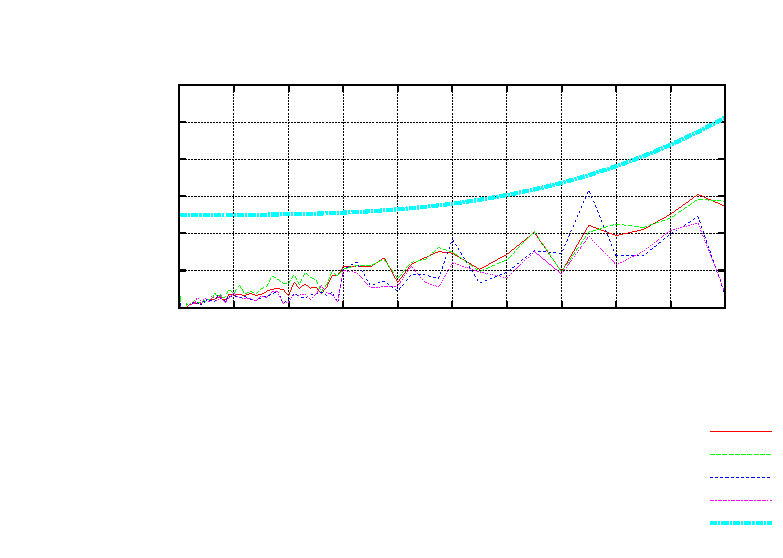
\includegraphics{ej3_nodos_nlogn_star+bridge+double_star}}%
    \gplfronttext
  \end{picture}%
\endgroup
}
    \caption{Complejidad temporal para grafos Estrella+Puente+Doble Estrella (Variante Max\_Iter=nlog(n))}
\end{figure}

\begin{figure}[H]
    \centering
    \fontsize{8}{10}\selectfont
    \resizebox{0.8\textwidth}{!}{% GNUPLOT: LaTeX picture with Postscript
\begingroup
  \makeatletter
  \providecommand\color[2][]{%
    \GenericError{(gnuplot) \space\space\space\@spaces}{%
      Package color not loaded in conjunction with
      terminal option `colourtext'%
    }{See the gnuplot documentation for explanation.%
    }{Either use 'blacktext' in gnuplot or load the package
      color.sty in LaTeX.}%
    \renewcommand\color[2][]{}%
  }%
  \providecommand\includegraphics[2][]{%
    \GenericError{(gnuplot) \space\space\space\@spaces}{%
      Package graphicx or graphics not loaded%
    }{See the gnuplot documentation for explanation.%
    }{The gnuplot epslatex terminal needs graphicx.sty or graphics.sty.}%
    \renewcommand\includegraphics[2][]{}%
  }%
  \providecommand\rotatebox[2]{#2}%
  \@ifundefined{ifGPcolor}{%
    \newif\ifGPcolor
    \GPcolortrue
  }{}%
  \@ifundefined{ifGPblacktext}{%
    \newif\ifGPblacktext
    \GPblacktexttrue
  }{}%
  % define a \g@addto@macro without @ in the name:
  \let\gplgaddtomacro\g@addto@macro
  % define empty templates for all commands taking text:
  \gdef\gplbacktext{}%
  \gdef\gplfronttext{}%
  \makeatother
  \ifGPblacktext
    % no textcolor at all
    \def\colorrgb#1{}%
    \def\colorgray#1{}%
  \else
    % gray or color?
    \ifGPcolor
      \def\colorrgb#1{\color[rgb]{#1}}%
      \def\colorgray#1{\color[gray]{#1}}%
      \expandafter\def\csname LTw\endcsname{\color{white}}%
      \expandafter\def\csname LTb\endcsname{\color{black}}%
      \expandafter\def\csname LTa\endcsname{\color{black}}%
      \expandafter\def\csname LT0\endcsname{\color[rgb]{1,0,0}}%
      \expandafter\def\csname LT1\endcsname{\color[rgb]{0,1,0}}%
      \expandafter\def\csname LT2\endcsname{\color[rgb]{0,0,1}}%
      \expandafter\def\csname LT3\endcsname{\color[rgb]{1,0,1}}%
      \expandafter\def\csname LT4\endcsname{\color[rgb]{0,1,1}}%
      \expandafter\def\csname LT5\endcsname{\color[rgb]{1,1,0}}%
      \expandafter\def\csname LT6\endcsname{\color[rgb]{0,0,0}}%
      \expandafter\def\csname LT7\endcsname{\color[rgb]{1,0.3,0}}%
      \expandafter\def\csname LT8\endcsname{\color[rgb]{0.5,0.5,0.5}}%
    \else
      % gray
      \def\colorrgb#1{\color{black}}%
      \def\colorgray#1{\color[gray]{#1}}%
      \expandafter\def\csname LTw\endcsname{\color{white}}%
      \expandafter\def\csname LTb\endcsname{\color{black}}%
      \expandafter\def\csname LTa\endcsname{\color{black}}%
      \expandafter\def\csname LT0\endcsname{\color{black}}%
      \expandafter\def\csname LT1\endcsname{\color{black}}%
      \expandafter\def\csname LT2\endcsname{\color{black}}%
      \expandafter\def\csname LT3\endcsname{\color{black}}%
      \expandafter\def\csname LT4\endcsname{\color{black}}%
      \expandafter\def\csname LT5\endcsname{\color{black}}%
      \expandafter\def\csname LT6\endcsname{\color{black}}%
      \expandafter\def\csname LT7\endcsname{\color{black}}%
      \expandafter\def\csname LT8\endcsname{\color{black}}%
    \fi
  \fi
  \setlength{\unitlength}{0.0500bp}%
  \begin{picture}(7200.00,5040.00)%
    \gplgaddtomacro\gplbacktext{%
      \csname LTb\endcsname%
      \put(1430,2244){\makebox(0,0)[r]{\strut{} 0}}%
      \csname LTb\endcsname%
      \put(1430,2458){\makebox(0,0)[r]{\strut{} 2000}}%
      \csname LTb\endcsname%
      \put(1430,2671){\makebox(0,0)[r]{\strut{} 4000}}%
      \csname LTb\endcsname%
      \put(1430,2885){\makebox(0,0)[r]{\strut{} 6000}}%
      \csname LTb\endcsname%
      \put(1430,3098){\makebox(0,0)[r]{\strut{} 8000}}%
      \csname LTb\endcsname%
      \put(1430,3312){\makebox(0,0)[r]{\strut{} 10000}}%
      \csname LTb\endcsname%
      \put(1430,3525){\makebox(0,0)[r]{\strut{} 12000}}%
      \csname LTb\endcsname%
      \put(1430,3739){\makebox(0,0)[r]{\strut{} 14000}}%
      \csname LTb\endcsname%
      \put(1430,3952){\makebox(0,0)[r]{\strut{} 16000}}%
      \csname LTb\endcsname%
      \put(1430,4166){\makebox(0,0)[r]{\strut{} 18000}}%
      \csname LTb\endcsname%
      \put(1430,4379){\makebox(0,0)[r]{\strut{} 20000}}%
      \csname LTb\endcsname%
      \put(1562,2024){\makebox(0,0){\strut{} 0}}%
      \csname LTb\endcsname%
      \put(2086,2024){\makebox(0,0){\strut{} 1000}}%
      \csname LTb\endcsname%
      \put(2610,2024){\makebox(0,0){\strut{} 2000}}%
      \csname LTb\endcsname%
      \put(3134,2024){\makebox(0,0){\strut{} 3000}}%
      \csname LTb\endcsname%
      \put(3658,2024){\makebox(0,0){\strut{} 4000}}%
      \csname LTb\endcsname%
      \put(4183,2024){\makebox(0,0){\strut{} 5000}}%
      \csname LTb\endcsname%
      \put(4707,2024){\makebox(0,0){\strut{} 6000}}%
      \csname LTb\endcsname%
      \put(5231,2024){\makebox(0,0){\strut{} 7000}}%
      \csname LTb\endcsname%
      \put(5755,2024){\makebox(0,0){\strut{} 8000}}%
      \csname LTb\endcsname%
      \put(6279,2024){\makebox(0,0){\strut{} 9000}}%
      \csname LTb\endcsname%
      \put(6803,2024){\makebox(0,0){\strut{} 10000}}%
      \put(176,3311){\rotatebox{-270}{\makebox(0,0){\strut{}Tiempo (microsegundos)}}}%
      \put(396,3311){\rotatebox{-270}{\makebox(0,0){\strut{}(Escala Lineal)}}}%
      \put(4182,1694){\makebox(0,0){\strut{}Cantidad de Nodos}}%
      \put(4182,1474){\makebox(0,0){\strut{}(Escala Lineal)}}%
      \put(4182,4709){\makebox(0,0){\strut{}Tiempo de ejecucion conforme aumenta la cantidad de nodos}}%
    }%
    \gplgaddtomacro\gplfronttext{%
      \csname LTb\endcsname%
      \put(6131,1053){\makebox(0,0)[r]{\strut{}Iter=n,Sin Mejorar=n,Tiempo Tabu=n}}%
      \csname LTb\endcsname%
      \put(6131,833){\makebox(0,0)[r]{\strut{}Iter=n,Sin Mejorar=n,Tiempo Tabu=n2}}%
      \csname LTb\endcsname%
      \put(6131,613){\makebox(0,0)[r]{\strut{}Iter=n,Sin Mejorar=n2,Tiempo Tabu=n}}%
      \csname LTb\endcsname%
      \put(6131,393){\makebox(0,0)[r]{\strut{}Iter=n,Sin Mejorar=n2,Tiempo Tabu=n2}}%
      \csname LTb\endcsname%
      \put(6131,173){\makebox(0,0)[r]{\strut{}Cota teórica superior $\mathcal O(n^3)$}}%
    }%
    \gplbacktext
    \put(0,0){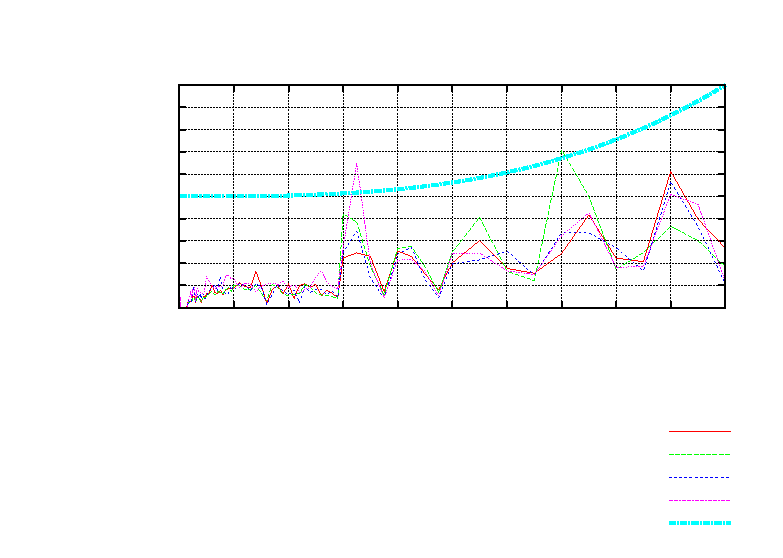
\includegraphics{ej3_nodos_n_star+bridge+double_star}}%
    \gplfronttext
  \end{picture}%
\endgroup
}
    \caption{Complejidad temporal para grafos Estrella+Puente+Doble Estrella (Variante Max\_Iter=n)}
\end{figure}

\begin{figure}[H]
    \centering
    \fontsize{8}{10}\selectfont
    \resizebox{0.8\textwidth}{!}{% GNUPLOT: LaTeX picture with Postscript
\begingroup
  \makeatletter
  \providecommand\color[2][]{%
    \GenericError{(gnuplot) \space\space\space\@spaces}{%
      Package color not loaded in conjunction with
      terminal option `colourtext'%
    }{See the gnuplot documentation for explanation.%
    }{Either use 'blacktext' in gnuplot or load the package
      color.sty in LaTeX.}%
    \renewcommand\color[2][]{}%
  }%
  \providecommand\includegraphics[2][]{%
    \GenericError{(gnuplot) \space\space\space\@spaces}{%
      Package graphicx or graphics not loaded%
    }{See the gnuplot documentation for explanation.%
    }{The gnuplot epslatex terminal needs graphicx.sty or graphics.sty.}%
    \renewcommand\includegraphics[2][]{}%
  }%
  \providecommand\rotatebox[2]{#2}%
  \@ifundefined{ifGPcolor}{%
    \newif\ifGPcolor
    \GPcolortrue
  }{}%
  \@ifundefined{ifGPblacktext}{%
    \newif\ifGPblacktext
    \GPblacktexttrue
  }{}%
  % define a \g@addto@macro without @ in the name:
  \let\gplgaddtomacro\g@addto@macro
  % define empty templates for all commands taking text:
  \gdef\gplbacktext{}%
  \gdef\gplfronttext{}%
  \makeatother
  \ifGPblacktext
    % no textcolor at all
    \def\colorrgb#1{}%
    \def\colorgray#1{}%
  \else
    % gray or color?
    \ifGPcolor
      \def\colorrgb#1{\color[rgb]{#1}}%
      \def\colorgray#1{\color[gray]{#1}}%
      \expandafter\def\csname LTw\endcsname{\color{white}}%
      \expandafter\def\csname LTb\endcsname{\color{black}}%
      \expandafter\def\csname LTa\endcsname{\color{black}}%
      \expandafter\def\csname LT0\endcsname{\color[rgb]{1,0,0}}%
      \expandafter\def\csname LT1\endcsname{\color[rgb]{0,1,0}}%
      \expandafter\def\csname LT2\endcsname{\color[rgb]{0,0,1}}%
      \expandafter\def\csname LT3\endcsname{\color[rgb]{1,0,1}}%
      \expandafter\def\csname LT4\endcsname{\color[rgb]{0,1,1}}%
      \expandafter\def\csname LT5\endcsname{\color[rgb]{1,1,0}}%
      \expandafter\def\csname LT6\endcsname{\color[rgb]{0,0,0}}%
      \expandafter\def\csname LT7\endcsname{\color[rgb]{1,0.3,0}}%
      \expandafter\def\csname LT8\endcsname{\color[rgb]{0.5,0.5,0.5}}%
    \else
      % gray
      \def\colorrgb#1{\color{black}}%
      \def\colorgray#1{\color[gray]{#1}}%
      \expandafter\def\csname LTw\endcsname{\color{white}}%
      \expandafter\def\csname LTb\endcsname{\color{black}}%
      \expandafter\def\csname LTa\endcsname{\color{black}}%
      \expandafter\def\csname LT0\endcsname{\color{black}}%
      \expandafter\def\csname LT1\endcsname{\color{black}}%
      \expandafter\def\csname LT2\endcsname{\color{black}}%
      \expandafter\def\csname LT3\endcsname{\color{black}}%
      \expandafter\def\csname LT4\endcsname{\color{black}}%
      \expandafter\def\csname LT5\endcsname{\color{black}}%
      \expandafter\def\csname LT6\endcsname{\color{black}}%
      \expandafter\def\csname LT7\endcsname{\color{black}}%
      \expandafter\def\csname LT8\endcsname{\color{black}}%
    \fi
  \fi
  \setlength{\unitlength}{0.0500bp}%
  \begin{picture}(7200.00,5040.00)%
    \gplgaddtomacro\gplbacktext{%
      \csname LTb\endcsname%
      \put(1034,3124){\makebox(0,0)[r]{\strut{} 1}}%
      \csname LTb\endcsname%
      \put(1034,3263){\makebox(0,0)[r]{\strut{} 2}}%
      \csname LTb\endcsname%
      \put(1034,3403){\makebox(0,0)[r]{\strut{} 3}}%
      \csname LTb\endcsname%
      \put(1034,3542){\makebox(0,0)[r]{\strut{} 4}}%
      \csname LTb\endcsname%
      \put(1034,3682){\makebox(0,0)[r]{\strut{} 5}}%
      \csname LTb\endcsname%
      \put(1034,3821){\makebox(0,0)[r]{\strut{} 6}}%
      \csname LTb\endcsname%
      \put(1034,3961){\makebox(0,0)[r]{\strut{} 7}}%
      \csname LTb\endcsname%
      \put(1034,4100){\makebox(0,0)[r]{\strut{} 8}}%
      \csname LTb\endcsname%
      \put(1034,4240){\makebox(0,0)[r]{\strut{} 9}}%
      \csname LTb\endcsname%
      \put(1034,4379){\makebox(0,0)[r]{\strut{} 10}}%
      \csname LTb\endcsname%
      \put(1166,2904){\makebox(0,0){\strut{} 0}}%
      \csname LTb\endcsname%
      \put(1730,2904){\makebox(0,0){\strut{} 1000}}%
      \csname LTb\endcsname%
      \put(2293,2904){\makebox(0,0){\strut{} 2000}}%
      \csname LTb\endcsname%
      \put(2857,2904){\makebox(0,0){\strut{} 3000}}%
      \csname LTb\endcsname%
      \put(3421,2904){\makebox(0,0){\strut{} 4000}}%
      \csname LTb\endcsname%
      \put(3985,2904){\makebox(0,0){\strut{} 5000}}%
      \csname LTb\endcsname%
      \put(4548,2904){\makebox(0,0){\strut{} 6000}}%
      \csname LTb\endcsname%
      \put(5112,2904){\makebox(0,0){\strut{} 7000}}%
      \csname LTb\endcsname%
      \put(5676,2904){\makebox(0,0){\strut{} 8000}}%
      \csname LTb\endcsname%
      \put(6239,2904){\makebox(0,0){\strut{} 9000}}%
      \csname LTb\endcsname%
      \put(6803,2904){\makebox(0,0){\strut{} 10000}}%
      \put(176,3751){\rotatebox{-270}{\makebox(0,0){\strut{}Frontera}}}%
      \put(396,3751){\rotatebox{-270}{\makebox(0,0){\strut{}(Escala Lineal)}}}%
      \put(3984,2574){\makebox(0,0){\strut{}Cantidad de Nodos}}%
      \put(3984,2354){\makebox(0,0){\strut{}(Escala Lineal)}}%
      \put(3984,4709){\makebox(0,0){\strut{}Frontera obtenida segun cantidad de nodos}}%
    }%
    \gplgaddtomacro\gplfronttext{%
      \csname LTb\endcsname%
      \put(6329,1933){\makebox(0,0)[r]{\strut{}Iter=nlog(n),Sin Mejorar=n,Tiempo Tabu=n}}%
      \csname LTb\endcsname%
      \put(6329,1713){\makebox(0,0)[r]{\strut{}Iter=nlog(n),Sin Mejorar=n,Tiempo Tabu=n2}}%
      \csname LTb\endcsname%
      \put(6329,1493){\makebox(0,0)[r]{\strut{}Iter=nlog(n),Sin Mejorar=n2,Tiempo Tabu=n}}%
      \csname LTb\endcsname%
      \put(6329,1273){\makebox(0,0)[r]{\strut{}Iter=nlog(n),Sin Mejorar=n2,Tiempo Tabu=n2}}%
      \csname LTb\endcsname%
      \put(6329,1053){\makebox(0,0)[r]{\strut{}Iter=n,Sin Mejorar=n,Tiempo Tabu=n}}%
      \csname LTb\endcsname%
      \put(6329,833){\makebox(0,0)[r]{\strut{}Iter=n,Sin Mejorar=n,Tiempo Tabu=n2}}%
      \csname LTb\endcsname%
      \put(6329,613){\makebox(0,0)[r]{\strut{}Iter=n,Sin Mejorar=n2,Tiempo Tabu=n}}%
      \csname LTb\endcsname%
      \put(6329,393){\makebox(0,0)[r]{\strut{}Iter=n,Sin Mejorar=n2,Tiempo Tabu=n2}}%
      \csname LTb\endcsname%
      \put(6329,173){\makebox(0,0)[r]{\strut{}Solucion optima}}%
    }%
    \gplbacktext
    \put(0,0){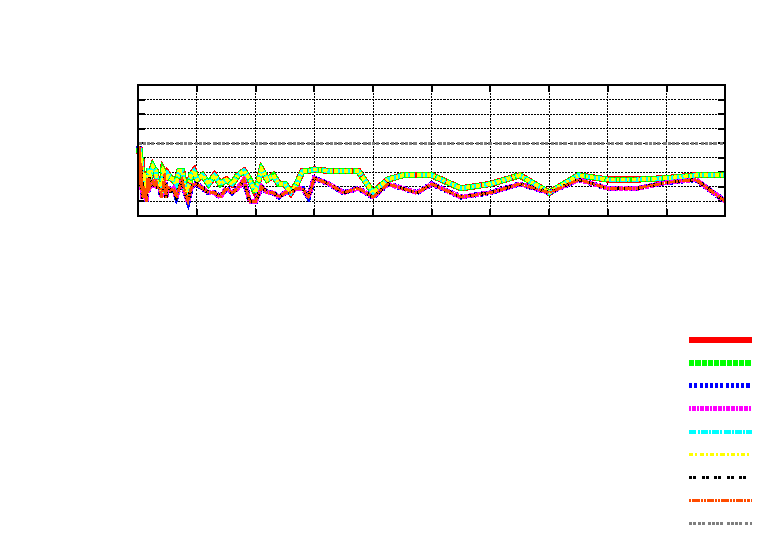
\includegraphics{ej3_frontera_star_bridge_double_star}}%
    \gplfronttext
  \end{picture}%
\endgroup
}
    \caption{Frontera de grafos Estrella+Puente+Doble Estrella}
\end{figure}

%Doble estrella sin aspiracion
\begin{figure}[H]
    \centering
    \fontsize{8}{10}\selectfont
    \resizebox{0.8\textwidth}{!}{% GNUPLOT: LaTeX picture with Postscript
\begingroup
  \makeatletter
  \providecommand\color[2][]{%
    \GenericError{(gnuplot) \space\space\space\@spaces}{%
      Package color not loaded in conjunction with
      terminal option `colourtext'%
    }{See the gnuplot documentation for explanation.%
    }{Either use 'blacktext' in gnuplot or load the package
      color.sty in LaTeX.}%
    \renewcommand\color[2][]{}%
  }%
  \providecommand\includegraphics[2][]{%
    \GenericError{(gnuplot) \space\space\space\@spaces}{%
      Package graphicx or graphics not loaded%
    }{See the gnuplot documentation for explanation.%
    }{The gnuplot epslatex terminal needs graphicx.sty or graphics.sty.}%
    \renewcommand\includegraphics[2][]{}%
  }%
  \providecommand\rotatebox[2]{#2}%
  \@ifundefined{ifGPcolor}{%
    \newif\ifGPcolor
    \GPcolortrue
  }{}%
  \@ifundefined{ifGPblacktext}{%
    \newif\ifGPblacktext
    \GPblacktexttrue
  }{}%
  % define a \g@addto@macro without @ in the name:
  \let\gplgaddtomacro\g@addto@macro
  % define empty templates for all commands taking text:
  \gdef\gplbacktext{}%
  \gdef\gplfronttext{}%
  \makeatother
  \ifGPblacktext
    % no textcolor at all
    \def\colorrgb#1{}%
    \def\colorgray#1{}%
  \else
    % gray or color?
    \ifGPcolor
      \def\colorrgb#1{\color[rgb]{#1}}%
      \def\colorgray#1{\color[gray]{#1}}%
      \expandafter\def\csname LTw\endcsname{\color{white}}%
      \expandafter\def\csname LTb\endcsname{\color{black}}%
      \expandafter\def\csname LTa\endcsname{\color{black}}%
      \expandafter\def\csname LT0\endcsname{\color[rgb]{1,0,0}}%
      \expandafter\def\csname LT1\endcsname{\color[rgb]{0,1,0}}%
      \expandafter\def\csname LT2\endcsname{\color[rgb]{0,0,1}}%
      \expandafter\def\csname LT3\endcsname{\color[rgb]{1,0,1}}%
      \expandafter\def\csname LT4\endcsname{\color[rgb]{0,1,1}}%
      \expandafter\def\csname LT5\endcsname{\color[rgb]{1,1,0}}%
      \expandafter\def\csname LT6\endcsname{\color[rgb]{0,0,0}}%
      \expandafter\def\csname LT7\endcsname{\color[rgb]{1,0.3,0}}%
      \expandafter\def\csname LT8\endcsname{\color[rgb]{0.5,0.5,0.5}}%
    \else
      % gray
      \def\colorrgb#1{\color{black}}%
      \def\colorgray#1{\color[gray]{#1}}%
      \expandafter\def\csname LTw\endcsname{\color{white}}%
      \expandafter\def\csname LTb\endcsname{\color{black}}%
      \expandafter\def\csname LTa\endcsname{\color{black}}%
      \expandafter\def\csname LT0\endcsname{\color{black}}%
      \expandafter\def\csname LT1\endcsname{\color{black}}%
      \expandafter\def\csname LT2\endcsname{\color{black}}%
      \expandafter\def\csname LT3\endcsname{\color{black}}%
      \expandafter\def\csname LT4\endcsname{\color{black}}%
      \expandafter\def\csname LT5\endcsname{\color{black}}%
      \expandafter\def\csname LT6\endcsname{\color{black}}%
      \expandafter\def\csname LT7\endcsname{\color{black}}%
      \expandafter\def\csname LT8\endcsname{\color{black}}%
    \fi
  \fi
  \setlength{\unitlength}{0.0500bp}%
  \begin{picture}(7200.00,5040.00)%
    \gplgaddtomacro\gplbacktext{%
      \csname LTb\endcsname%
      \put(1430,2244){\makebox(0,0)[r]{\strut{} 0}}%
      \csname LTb\endcsname%
      \put(1430,2600){\makebox(0,0)[r]{\strut{} 10000}}%
      \csname LTb\endcsname%
      \put(1430,2956){\makebox(0,0)[r]{\strut{} 20000}}%
      \csname LTb\endcsname%
      \put(1430,3312){\makebox(0,0)[r]{\strut{} 30000}}%
      \csname LTb\endcsname%
      \put(1430,3667){\makebox(0,0)[r]{\strut{} 40000}}%
      \csname LTb\endcsname%
      \put(1430,4023){\makebox(0,0)[r]{\strut{} 50000}}%
      \csname LTb\endcsname%
      \put(1430,4379){\makebox(0,0)[r]{\strut{} 60000}}%
      \csname LTb\endcsname%
      \put(1562,2024){\makebox(0,0){\strut{} 0}}%
      \csname LTb\endcsname%
      \put(2086,2024){\makebox(0,0){\strut{} 1000}}%
      \csname LTb\endcsname%
      \put(2610,2024){\makebox(0,0){\strut{} 2000}}%
      \csname LTb\endcsname%
      \put(3134,2024){\makebox(0,0){\strut{} 3000}}%
      \csname LTb\endcsname%
      \put(3658,2024){\makebox(0,0){\strut{} 4000}}%
      \csname LTb\endcsname%
      \put(4183,2024){\makebox(0,0){\strut{} 5000}}%
      \csname LTb\endcsname%
      \put(4707,2024){\makebox(0,0){\strut{} 6000}}%
      \csname LTb\endcsname%
      \put(5231,2024){\makebox(0,0){\strut{} 7000}}%
      \csname LTb\endcsname%
      \put(5755,2024){\makebox(0,0){\strut{} 8000}}%
      \csname LTb\endcsname%
      \put(6279,2024){\makebox(0,0){\strut{} 9000}}%
      \csname LTb\endcsname%
      \put(6803,2024){\makebox(0,0){\strut{} 10000}}%
      \put(176,3311){\rotatebox{-270}{\makebox(0,0){\strut{}Tiempo (microsegundos)}}}%
      \put(396,3311){\rotatebox{-270}{\makebox(0,0){\strut{}(Escala Lineal)}}}%
      \put(4182,1694){\makebox(0,0){\strut{}Cantidad de Nodos}}%
      \put(4182,1474){\makebox(0,0){\strut{}(Escala Lineal)}}%
      \put(4182,4709){\makebox(0,0){\strut{}Tiempo de ejecucion conforme aumenta la cantidad de nodos}}%
    }%
    \gplgaddtomacro\gplfronttext{%
      \csname LTb\endcsname%
      \put(6527,1053){\makebox(0,0)[r]{\strut{}Iter=nlog(n),Sin Mejorar=n,Tiempo Tabu=n}}%
      \csname LTb\endcsname%
      \put(6527,833){\makebox(0,0)[r]{\strut{}Iter=nlog(n),Sin Mejorar=n,Tiempo Tabu=n2}}%
      \csname LTb\endcsname%
      \put(6527,613){\makebox(0,0)[r]{\strut{}Iter=nlog(n),Sin Mejorar=n2,Tiempo Tabu=n}}%
      \csname LTb\endcsname%
      \put(6527,393){\makebox(0,0)[r]{\strut{}Iter=nlog(n),Sin Mejorar=n2,Tiempo Tabu=n2}}%
      \csname LTb\endcsname%
      \put(6527,173){\makebox(0,0)[r]{\strut{}Cota teórica superior $\mathcal O(n^3 \cdot log(n))$}}%
    }%
    \gplbacktext
    \put(0,0){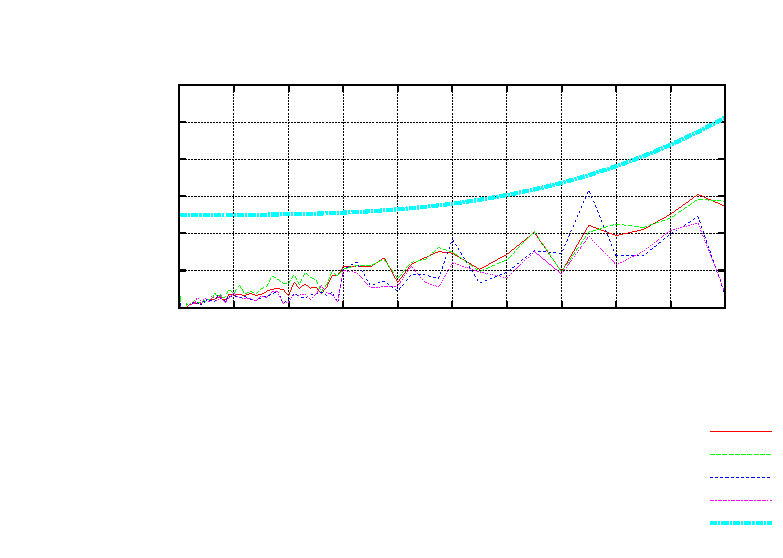
\includegraphics{ej3_nodos_nlogn_star+bridge+double_star_sin_aspiracion}}%
    \gplfronttext
  \end{picture}%
\endgroup
}
    \caption{Complejidad temporal para grafos Estrella+Puente+Doble Estrella (Variante Max\_Iter=nlog(n),sin aspiraci\'on)}
\end{figure}

\begin{figure}[H]
    \centering
    \fontsize{8}{10}\selectfont
    \resizebox{0.8\textwidth}{!}{% GNUPLOT: LaTeX picture with Postscript
\begingroup
  \makeatletter
  \providecommand\color[2][]{%
    \GenericError{(gnuplot) \space\space\space\@spaces}{%
      Package color not loaded in conjunction with
      terminal option `colourtext'%
    }{See the gnuplot documentation for explanation.%
    }{Either use 'blacktext' in gnuplot or load the package
      color.sty in LaTeX.}%
    \renewcommand\color[2][]{}%
  }%
  \providecommand\includegraphics[2][]{%
    \GenericError{(gnuplot) \space\space\space\@spaces}{%
      Package graphicx or graphics not loaded%
    }{See the gnuplot documentation for explanation.%
    }{The gnuplot epslatex terminal needs graphicx.sty or graphics.sty.}%
    \renewcommand\includegraphics[2][]{}%
  }%
  \providecommand\rotatebox[2]{#2}%
  \@ifundefined{ifGPcolor}{%
    \newif\ifGPcolor
    \GPcolortrue
  }{}%
  \@ifundefined{ifGPblacktext}{%
    \newif\ifGPblacktext
    \GPblacktexttrue
  }{}%
  % define a \g@addto@macro without @ in the name:
  \let\gplgaddtomacro\g@addto@macro
  % define empty templates for all commands taking text:
  \gdef\gplbacktext{}%
  \gdef\gplfronttext{}%
  \makeatother
  \ifGPblacktext
    % no textcolor at all
    \def\colorrgb#1{}%
    \def\colorgray#1{}%
  \else
    % gray or color?
    \ifGPcolor
      \def\colorrgb#1{\color[rgb]{#1}}%
      \def\colorgray#1{\color[gray]{#1}}%
      \expandafter\def\csname LTw\endcsname{\color{white}}%
      \expandafter\def\csname LTb\endcsname{\color{black}}%
      \expandafter\def\csname LTa\endcsname{\color{black}}%
      \expandafter\def\csname LT0\endcsname{\color[rgb]{1,0,0}}%
      \expandafter\def\csname LT1\endcsname{\color[rgb]{0,1,0}}%
      \expandafter\def\csname LT2\endcsname{\color[rgb]{0,0,1}}%
      \expandafter\def\csname LT3\endcsname{\color[rgb]{1,0,1}}%
      \expandafter\def\csname LT4\endcsname{\color[rgb]{0,1,1}}%
      \expandafter\def\csname LT5\endcsname{\color[rgb]{1,1,0}}%
      \expandafter\def\csname LT6\endcsname{\color[rgb]{0,0,0}}%
      \expandafter\def\csname LT7\endcsname{\color[rgb]{1,0.3,0}}%
      \expandafter\def\csname LT8\endcsname{\color[rgb]{0.5,0.5,0.5}}%
    \else
      % gray
      \def\colorrgb#1{\color{black}}%
      \def\colorgray#1{\color[gray]{#1}}%
      \expandafter\def\csname LTw\endcsname{\color{white}}%
      \expandafter\def\csname LTb\endcsname{\color{black}}%
      \expandafter\def\csname LTa\endcsname{\color{black}}%
      \expandafter\def\csname LT0\endcsname{\color{black}}%
      \expandafter\def\csname LT1\endcsname{\color{black}}%
      \expandafter\def\csname LT2\endcsname{\color{black}}%
      \expandafter\def\csname LT3\endcsname{\color{black}}%
      \expandafter\def\csname LT4\endcsname{\color{black}}%
      \expandafter\def\csname LT5\endcsname{\color{black}}%
      \expandafter\def\csname LT6\endcsname{\color{black}}%
      \expandafter\def\csname LT7\endcsname{\color{black}}%
      \expandafter\def\csname LT8\endcsname{\color{black}}%
    \fi
  \fi
  \setlength{\unitlength}{0.0500bp}%
  \begin{picture}(7200.00,5040.00)%
    \gplgaddtomacro\gplbacktext{%
      \csname LTb\endcsname%
      \put(1430,2244){\makebox(0,0)[r]{\strut{} 0}}%
      \csname LTb\endcsname%
      \put(1430,2458){\makebox(0,0)[r]{\strut{} 2000}}%
      \csname LTb\endcsname%
      \put(1430,2671){\makebox(0,0)[r]{\strut{} 4000}}%
      \csname LTb\endcsname%
      \put(1430,2885){\makebox(0,0)[r]{\strut{} 6000}}%
      \csname LTb\endcsname%
      \put(1430,3098){\makebox(0,0)[r]{\strut{} 8000}}%
      \csname LTb\endcsname%
      \put(1430,3312){\makebox(0,0)[r]{\strut{} 10000}}%
      \csname LTb\endcsname%
      \put(1430,3525){\makebox(0,0)[r]{\strut{} 12000}}%
      \csname LTb\endcsname%
      \put(1430,3739){\makebox(0,0)[r]{\strut{} 14000}}%
      \csname LTb\endcsname%
      \put(1430,3952){\makebox(0,0)[r]{\strut{} 16000}}%
      \csname LTb\endcsname%
      \put(1430,4166){\makebox(0,0)[r]{\strut{} 18000}}%
      \csname LTb\endcsname%
      \put(1430,4379){\makebox(0,0)[r]{\strut{} 20000}}%
      \csname LTb\endcsname%
      \put(1562,2024){\makebox(0,0){\strut{} 0}}%
      \csname LTb\endcsname%
      \put(2086,2024){\makebox(0,0){\strut{} 1000}}%
      \csname LTb\endcsname%
      \put(2610,2024){\makebox(0,0){\strut{} 2000}}%
      \csname LTb\endcsname%
      \put(3134,2024){\makebox(0,0){\strut{} 3000}}%
      \csname LTb\endcsname%
      \put(3658,2024){\makebox(0,0){\strut{} 4000}}%
      \csname LTb\endcsname%
      \put(4183,2024){\makebox(0,0){\strut{} 5000}}%
      \csname LTb\endcsname%
      \put(4707,2024){\makebox(0,0){\strut{} 6000}}%
      \csname LTb\endcsname%
      \put(5231,2024){\makebox(0,0){\strut{} 7000}}%
      \csname LTb\endcsname%
      \put(5755,2024){\makebox(0,0){\strut{} 8000}}%
      \csname LTb\endcsname%
      \put(6279,2024){\makebox(0,0){\strut{} 9000}}%
      \csname LTb\endcsname%
      \put(6803,2024){\makebox(0,0){\strut{} 10000}}%
      \put(176,3311){\rotatebox{-270}{\makebox(0,0){\strut{}Tiempo (microsegundos)}}}%
      \put(396,3311){\rotatebox{-270}{\makebox(0,0){\strut{}(Escala Lineal)}}}%
      \put(4182,1694){\makebox(0,0){\strut{}Cantidad de Nodos}}%
      \put(4182,1474){\makebox(0,0){\strut{}(Escala Lineal)}}%
      \put(4182,4709){\makebox(0,0){\strut{}Tiempo de ejecucion conforme aumenta la cantidad de nodos}}%
    }%
    \gplgaddtomacro\gplfronttext{%
      \csname LTb\endcsname%
      \put(6131,1053){\makebox(0,0)[r]{\strut{}Iter=n,Sin Mejorar=n,Tiempo Tabu=n}}%
      \csname LTb\endcsname%
      \put(6131,833){\makebox(0,0)[r]{\strut{}Iter=n,Sin Mejorar=n,Tiempo Tabu=n2}}%
      \csname LTb\endcsname%
      \put(6131,613){\makebox(0,0)[r]{\strut{}Iter=n,Sin Mejorar=n2,Tiempo Tabu=n}}%
      \csname LTb\endcsname%
      \put(6131,393){\makebox(0,0)[r]{\strut{}Iter=n,Sin Mejorar=n2,Tiempo Tabu=n2}}%
      \csname LTb\endcsname%
      \put(6131,173){\makebox(0,0)[r]{\strut{}Cota teórica superior $\mathcal O(n^3)$}}%
    }%
    \gplbacktext
    \put(0,0){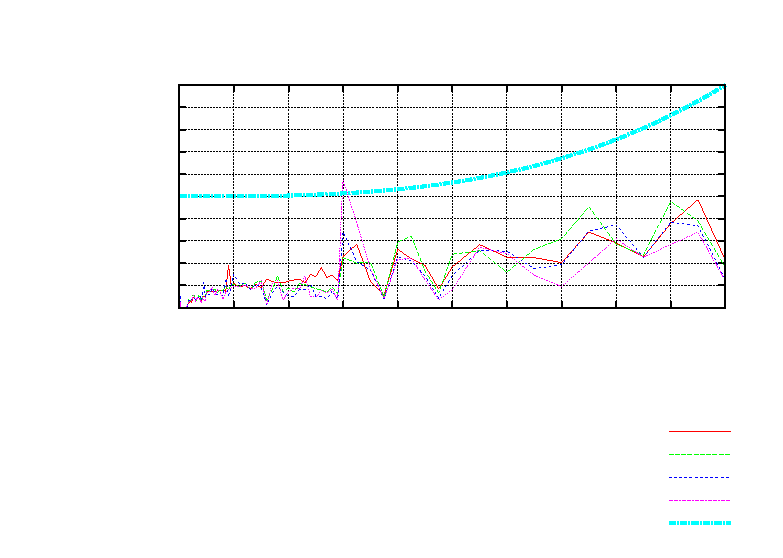
\includegraphics{ej3_nodos_n_star+bridge+double_star_sin_aspiracion}}%
    \gplfronttext
  \end{picture}%
\endgroup
}
    \caption{Complejidad temporal para grafos Estrella+Puente+Doble Estrella (Variante Max\_Iter=n),sin aspiraci\'on)}
\end{figure}

\begin{figure}[H]
    \centering
    \fontsize{8}{10}\selectfont
    \resizebox{0.8\textwidth}{!}{% GNUPLOT: LaTeX picture with Postscript
\begingroup
  \makeatletter
  \providecommand\color[2][]{%
    \GenericError{(gnuplot) \space\space\space\@spaces}{%
      Package color not loaded in conjunction with
      terminal option `colourtext'%
    }{See the gnuplot documentation for explanation.%
    }{Either use 'blacktext' in gnuplot or load the package
      color.sty in LaTeX.}%
    \renewcommand\color[2][]{}%
  }%
  \providecommand\includegraphics[2][]{%
    \GenericError{(gnuplot) \space\space\space\@spaces}{%
      Package graphicx or graphics not loaded%
    }{See the gnuplot documentation for explanation.%
    }{The gnuplot epslatex terminal needs graphicx.sty or graphics.sty.}%
    \renewcommand\includegraphics[2][]{}%
  }%
  \providecommand\rotatebox[2]{#2}%
  \@ifundefined{ifGPcolor}{%
    \newif\ifGPcolor
    \GPcolortrue
  }{}%
  \@ifundefined{ifGPblacktext}{%
    \newif\ifGPblacktext
    \GPblacktexttrue
  }{}%
  % define a \g@addto@macro without @ in the name:
  \let\gplgaddtomacro\g@addto@macro
  % define empty templates for all commands taking text:
  \gdef\gplbacktext{}%
  \gdef\gplfronttext{}%
  \makeatother
  \ifGPblacktext
    % no textcolor at all
    \def\colorrgb#1{}%
    \def\colorgray#1{}%
  \else
    % gray or color?
    \ifGPcolor
      \def\colorrgb#1{\color[rgb]{#1}}%
      \def\colorgray#1{\color[gray]{#1}}%
      \expandafter\def\csname LTw\endcsname{\color{white}}%
      \expandafter\def\csname LTb\endcsname{\color{black}}%
      \expandafter\def\csname LTa\endcsname{\color{black}}%
      \expandafter\def\csname LT0\endcsname{\color[rgb]{1,0,0}}%
      \expandafter\def\csname LT1\endcsname{\color[rgb]{0,1,0}}%
      \expandafter\def\csname LT2\endcsname{\color[rgb]{0,0,1}}%
      \expandafter\def\csname LT3\endcsname{\color[rgb]{1,0,1}}%
      \expandafter\def\csname LT4\endcsname{\color[rgb]{0,1,1}}%
      \expandafter\def\csname LT5\endcsname{\color[rgb]{1,1,0}}%
      \expandafter\def\csname LT6\endcsname{\color[rgb]{0,0,0}}%
      \expandafter\def\csname LT7\endcsname{\color[rgb]{1,0.3,0}}%
      \expandafter\def\csname LT8\endcsname{\color[rgb]{0.5,0.5,0.5}}%
    \else
      % gray
      \def\colorrgb#1{\color{black}}%
      \def\colorgray#1{\color[gray]{#1}}%
      \expandafter\def\csname LTw\endcsname{\color{white}}%
      \expandafter\def\csname LTb\endcsname{\color{black}}%
      \expandafter\def\csname LTa\endcsname{\color{black}}%
      \expandafter\def\csname LT0\endcsname{\color{black}}%
      \expandafter\def\csname LT1\endcsname{\color{black}}%
      \expandafter\def\csname LT2\endcsname{\color{black}}%
      \expandafter\def\csname LT3\endcsname{\color{black}}%
      \expandafter\def\csname LT4\endcsname{\color{black}}%
      \expandafter\def\csname LT5\endcsname{\color{black}}%
      \expandafter\def\csname LT6\endcsname{\color{black}}%
      \expandafter\def\csname LT7\endcsname{\color{black}}%
      \expandafter\def\csname LT8\endcsname{\color{black}}%
    \fi
  \fi
  \setlength{\unitlength}{0.0500bp}%
  \begin{picture}(7200.00,5040.00)%
    \gplgaddtomacro\gplbacktext{%
      \csname LTb\endcsname%
      \put(1034,3124){\makebox(0,0)[r]{\strut{} 1}}%
      \csname LTb\endcsname%
      \put(1034,3263){\makebox(0,0)[r]{\strut{} 2}}%
      \csname LTb\endcsname%
      \put(1034,3403){\makebox(0,0)[r]{\strut{} 3}}%
      \csname LTb\endcsname%
      \put(1034,3542){\makebox(0,0)[r]{\strut{} 4}}%
      \csname LTb\endcsname%
      \put(1034,3682){\makebox(0,0)[r]{\strut{} 5}}%
      \csname LTb\endcsname%
      \put(1034,3821){\makebox(0,0)[r]{\strut{} 6}}%
      \csname LTb\endcsname%
      \put(1034,3961){\makebox(0,0)[r]{\strut{} 7}}%
      \csname LTb\endcsname%
      \put(1034,4100){\makebox(0,0)[r]{\strut{} 8}}%
      \csname LTb\endcsname%
      \put(1034,4240){\makebox(0,0)[r]{\strut{} 9}}%
      \csname LTb\endcsname%
      \put(1034,4379){\makebox(0,0)[r]{\strut{} 10}}%
      \csname LTb\endcsname%
      \put(1166,2904){\makebox(0,0){\strut{} 0}}%
      \csname LTb\endcsname%
      \put(1730,2904){\makebox(0,0){\strut{} 1000}}%
      \csname LTb\endcsname%
      \put(2293,2904){\makebox(0,0){\strut{} 2000}}%
      \csname LTb\endcsname%
      \put(2857,2904){\makebox(0,0){\strut{} 3000}}%
      \csname LTb\endcsname%
      \put(3421,2904){\makebox(0,0){\strut{} 4000}}%
      \csname LTb\endcsname%
      \put(3985,2904){\makebox(0,0){\strut{} 5000}}%
      \csname LTb\endcsname%
      \put(4548,2904){\makebox(0,0){\strut{} 6000}}%
      \csname LTb\endcsname%
      \put(5112,2904){\makebox(0,0){\strut{} 7000}}%
      \csname LTb\endcsname%
      \put(5676,2904){\makebox(0,0){\strut{} 8000}}%
      \csname LTb\endcsname%
      \put(6239,2904){\makebox(0,0){\strut{} 9000}}%
      \csname LTb\endcsname%
      \put(6803,2904){\makebox(0,0){\strut{} 10000}}%
      \put(176,3751){\rotatebox{-270}{\makebox(0,0){\strut{}Frontera}}}%
      \put(396,3751){\rotatebox{-270}{\makebox(0,0){\strut{}(Escala Lineal)}}}%
      \put(3984,2574){\makebox(0,0){\strut{}Cantidad de Nodos}}%
      \put(3984,2354){\makebox(0,0){\strut{}(Escala Lineal)}}%
      \put(3984,4709){\makebox(0,0){\strut{}Frontera obtenida segun cantidad de nodos}}%
    }%
    \gplgaddtomacro\gplfronttext{%
      \csname LTb\endcsname%
      \put(6329,1933){\makebox(0,0)[r]{\strut{}Iter=nlog(n),Sin Mejorar=n,Tiempo Tabu=n}}%
      \csname LTb\endcsname%
      \put(6329,1713){\makebox(0,0)[r]{\strut{}Iter=nlog(n),Sin Mejorar=n,Tiempo Tabu=n2}}%
      \csname LTb\endcsname%
      \put(6329,1493){\makebox(0,0)[r]{\strut{}Iter=nlog(n),Sin Mejorar=n2,Tiempo Tabu=n}}%
      \csname LTb\endcsname%
      \put(6329,1273){\makebox(0,0)[r]{\strut{}Iter=nlog(n),Sin Mejorar=n2,Tiempo Tabu=n2}}%
      \csname LTb\endcsname%
      \put(6329,1053){\makebox(0,0)[r]{\strut{}Iter=n,Sin Mejorar=n,Tiempo Tabu=n}}%
      \csname LTb\endcsname%
      \put(6329,833){\makebox(0,0)[r]{\strut{}Iter=n,Sin Mejorar=n,Tiempo Tabu=n2}}%
      \csname LTb\endcsname%
      \put(6329,613){\makebox(0,0)[r]{\strut{}Iter=n,Sin Mejorar=n2,Tiempo Tabu=n}}%
      \csname LTb\endcsname%
      \put(6329,393){\makebox(0,0)[r]{\strut{}Iter=n,Sin Mejorar=n2,Tiempo Tabu=n2}}%
      \csname LTb\endcsname%
      \put(6329,173){\makebox(0,0)[r]{\strut{}Solucion optima}}%
    }%
    \gplbacktext
    \put(0,0){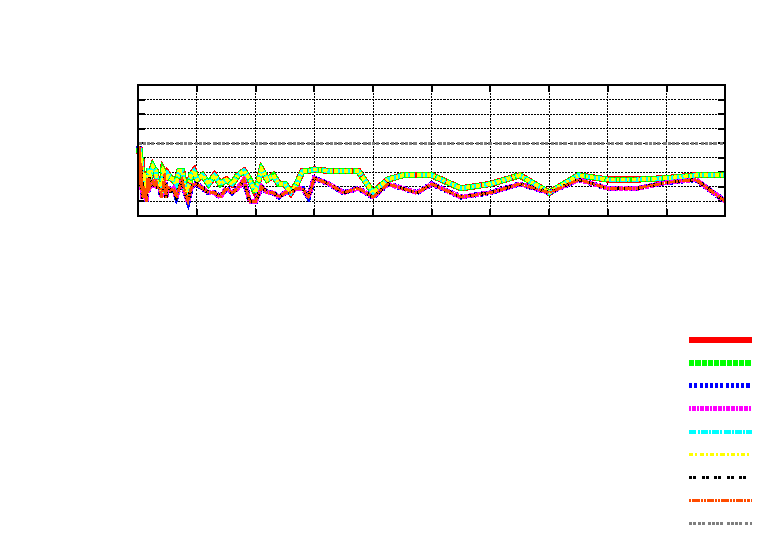
\includegraphics{ej3_frontera_star_bridge_double_star_sin_aspiracion}}%
    \gplfronttext
  \end{picture}%
\endgroup
}
    \caption{Frontera de grafos Estrella+Puente+Doble Estrella (sin aspiracion)}
\end{figure}

%Doble estrella sin aspiracion golosa
\begin{figure}[H]
    \centering
    \fontsize{8}{10}\selectfont
    \resizebox{0.8\textwidth}{!}{% GNUPLOT: LaTeX picture with Postscript
\begingroup
  \makeatletter
  \providecommand\color[2][]{%
    \GenericError{(gnuplot) \space\space\space\@spaces}{%
      Package color not loaded in conjunction with
      terminal option `colourtext'%
    }{See the gnuplot documentation for explanation.%
    }{Either use 'blacktext' in gnuplot or load the package
      color.sty in LaTeX.}%
    \renewcommand\color[2][]{}%
  }%
  \providecommand\includegraphics[2][]{%
    \GenericError{(gnuplot) \space\space\space\@spaces}{%
      Package graphicx or graphics not loaded%
    }{See the gnuplot documentation for explanation.%
    }{The gnuplot epslatex terminal needs graphicx.sty or graphics.sty.}%
    \renewcommand\includegraphics[2][]{}%
  }%
  \providecommand\rotatebox[2]{#2}%
  \@ifundefined{ifGPcolor}{%
    \newif\ifGPcolor
    \GPcolortrue
  }{}%
  \@ifundefined{ifGPblacktext}{%
    \newif\ifGPblacktext
    \GPblacktexttrue
  }{}%
  % define a \g@addto@macro without @ in the name:
  \let\gplgaddtomacro\g@addto@macro
  % define empty templates for all commands taking text:
  \gdef\gplbacktext{}%
  \gdef\gplfronttext{}%
  \makeatother
  \ifGPblacktext
    % no textcolor at all
    \def\colorrgb#1{}%
    \def\colorgray#1{}%
  \else
    % gray or color?
    \ifGPcolor
      \def\colorrgb#1{\color[rgb]{#1}}%
      \def\colorgray#1{\color[gray]{#1}}%
      \expandafter\def\csname LTw\endcsname{\color{white}}%
      \expandafter\def\csname LTb\endcsname{\color{black}}%
      \expandafter\def\csname LTa\endcsname{\color{black}}%
      \expandafter\def\csname LT0\endcsname{\color[rgb]{1,0,0}}%
      \expandafter\def\csname LT1\endcsname{\color[rgb]{0,1,0}}%
      \expandafter\def\csname LT2\endcsname{\color[rgb]{0,0,1}}%
      \expandafter\def\csname LT3\endcsname{\color[rgb]{1,0,1}}%
      \expandafter\def\csname LT4\endcsname{\color[rgb]{0,1,1}}%
      \expandafter\def\csname LT5\endcsname{\color[rgb]{1,1,0}}%
      \expandafter\def\csname LT6\endcsname{\color[rgb]{0,0,0}}%
      \expandafter\def\csname LT7\endcsname{\color[rgb]{1,0.3,0}}%
      \expandafter\def\csname LT8\endcsname{\color[rgb]{0.5,0.5,0.5}}%
    \else
      % gray
      \def\colorrgb#1{\color{black}}%
      \def\colorgray#1{\color[gray]{#1}}%
      \expandafter\def\csname LTw\endcsname{\color{white}}%
      \expandafter\def\csname LTb\endcsname{\color{black}}%
      \expandafter\def\csname LTa\endcsname{\color{black}}%
      \expandafter\def\csname LT0\endcsname{\color{black}}%
      \expandafter\def\csname LT1\endcsname{\color{black}}%
      \expandafter\def\csname LT2\endcsname{\color{black}}%
      \expandafter\def\csname LT3\endcsname{\color{black}}%
      \expandafter\def\csname LT4\endcsname{\color{black}}%
      \expandafter\def\csname LT5\endcsname{\color{black}}%
      \expandafter\def\csname LT6\endcsname{\color{black}}%
      \expandafter\def\csname LT7\endcsname{\color{black}}%
      \expandafter\def\csname LT8\endcsname{\color{black}}%
    \fi
  \fi
  \setlength{\unitlength}{0.0500bp}%
  \begin{picture}(7200.00,5040.00)%
    \gplgaddtomacro\gplbacktext{%
      \csname LTb\endcsname%
      \put(1562,2244){\makebox(0,0)[r]{\strut{} 0}}%
      \csname LTb\endcsname%
      \put(1562,2600){\makebox(0,0)[r]{\strut{} 20000}}%
      \csname LTb\endcsname%
      \put(1562,2956){\makebox(0,0)[r]{\strut{} 40000}}%
      \csname LTb\endcsname%
      \put(1562,3312){\makebox(0,0)[r]{\strut{} 60000}}%
      \csname LTb\endcsname%
      \put(1562,3667){\makebox(0,0)[r]{\strut{} 80000}}%
      \csname LTb\endcsname%
      \put(1562,4023){\makebox(0,0)[r]{\strut{} 100000}}%
      \csname LTb\endcsname%
      \put(1562,4379){\makebox(0,0)[r]{\strut{} 120000}}%
      \csname LTb\endcsname%
      \put(1694,2024){\makebox(0,0){\strut{} 0}}%
      \csname LTb\endcsname%
      \put(2205,2024){\makebox(0,0){\strut{} 1000}}%
      \csname LTb\endcsname%
      \put(2716,2024){\makebox(0,0){\strut{} 2000}}%
      \csname LTb\endcsname%
      \put(3227,2024){\makebox(0,0){\strut{} 3000}}%
      \csname LTb\endcsname%
      \put(3738,2024){\makebox(0,0){\strut{} 4000}}%
      \csname LTb\endcsname%
      \put(4249,2024){\makebox(0,0){\strut{} 5000}}%
      \csname LTb\endcsname%
      \put(4759,2024){\makebox(0,0){\strut{} 6000}}%
      \csname LTb\endcsname%
      \put(5270,2024){\makebox(0,0){\strut{} 7000}}%
      \csname LTb\endcsname%
      \put(5781,2024){\makebox(0,0){\strut{} 8000}}%
      \csname LTb\endcsname%
      \put(6292,2024){\makebox(0,0){\strut{} 9000}}%
      \csname LTb\endcsname%
      \put(6803,2024){\makebox(0,0){\strut{} 10000}}%
      \put(176,3311){\rotatebox{-270}{\makebox(0,0){\strut{}Tiempo (microsegundos)}}}%
      \put(396,3311){\rotatebox{-270}{\makebox(0,0){\strut{}(Escala Lineal)}}}%
      \put(4248,1694){\makebox(0,0){\strut{}Cantidad de Nodos}}%
      \put(4248,1474){\makebox(0,0){\strut{}(Escala Lineal)}}%
      \put(4248,4709){\makebox(0,0){\strut{}Tiempo de ejecucion conforme aumenta la cantidad de nodos}}%
    }%
    \gplgaddtomacro\gplfronttext{%
      \csname LTb\endcsname%
      \put(6593,1053){\makebox(0,0)[r]{\strut{}Iter=nlog(n),Sin Mejorar=n,Tiempo Tabu=n}}%
      \csname LTb\endcsname%
      \put(6593,833){\makebox(0,0)[r]{\strut{}Iter=nlog(n),Sin Mejorar=n,Tiempo Tabu=n2}}%
      \csname LTb\endcsname%
      \put(6593,613){\makebox(0,0)[r]{\strut{}Iter=nlog(n),Sin Mejorar=n2,Tiempo Tabu=n}}%
      \csname LTb\endcsname%
      \put(6593,393){\makebox(0,0)[r]{\strut{}Iter=nlog(n),Sin Mejorar=n2,Tiempo Tabu=n2}}%
      \csname LTb\endcsname%
      \put(6593,173){\makebox(0,0)[r]{\strut{}Cota teórica superior $\mathcal O(n^3 \cdot log(n))$}}%
    }%
    \gplbacktext
    \put(0,0){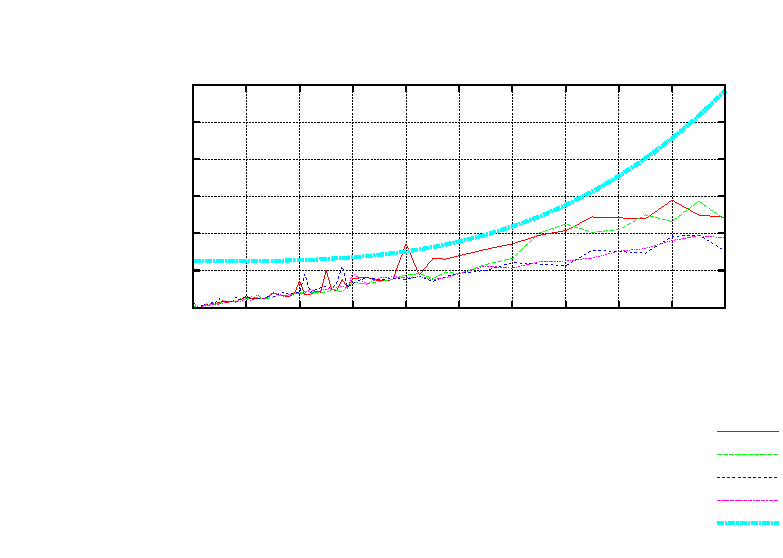
\includegraphics{ej3_nodos_nlogn_star+bridge+double_star_sin_aspiracion_golosa}}%
    \gplfronttext
  \end{picture}%
\endgroup
}
    \caption{Complejidad temporal para grafos Estrella+Puente+Doble Estrella (Variante Max\_Iter=nlog(n),sin aspiraci\'on,golosa)}
\end{figure}

\begin{figure}[H]
    \centering
    \fontsize{8}{10}\selectfont
    \resizebox{0.8\textwidth}{!}{% GNUPLOT: LaTeX picture with Postscript
\begingroup
  \makeatletter
  \providecommand\color[2][]{%
    \GenericError{(gnuplot) \space\space\space\@spaces}{%
      Package color not loaded in conjunction with
      terminal option `colourtext'%
    }{See the gnuplot documentation for explanation.%
    }{Either use 'blacktext' in gnuplot or load the package
      color.sty in LaTeX.}%
    \renewcommand\color[2][]{}%
  }%
  \providecommand\includegraphics[2][]{%
    \GenericError{(gnuplot) \space\space\space\@spaces}{%
      Package graphicx or graphics not loaded%
    }{See the gnuplot documentation for explanation.%
    }{The gnuplot epslatex terminal needs graphicx.sty or graphics.sty.}%
    \renewcommand\includegraphics[2][]{}%
  }%
  \providecommand\rotatebox[2]{#2}%
  \@ifundefined{ifGPcolor}{%
    \newif\ifGPcolor
    \GPcolortrue
  }{}%
  \@ifundefined{ifGPblacktext}{%
    \newif\ifGPblacktext
    \GPblacktexttrue
  }{}%
  % define a \g@addto@macro without @ in the name:
  \let\gplgaddtomacro\g@addto@macro
  % define empty templates for all commands taking text:
  \gdef\gplbacktext{}%
  \gdef\gplfronttext{}%
  \makeatother
  \ifGPblacktext
    % no textcolor at all
    \def\colorrgb#1{}%
    \def\colorgray#1{}%
  \else
    % gray or color?
    \ifGPcolor
      \def\colorrgb#1{\color[rgb]{#1}}%
      \def\colorgray#1{\color[gray]{#1}}%
      \expandafter\def\csname LTw\endcsname{\color{white}}%
      \expandafter\def\csname LTb\endcsname{\color{black}}%
      \expandafter\def\csname LTa\endcsname{\color{black}}%
      \expandafter\def\csname LT0\endcsname{\color[rgb]{1,0,0}}%
      \expandafter\def\csname LT1\endcsname{\color[rgb]{0,1,0}}%
      \expandafter\def\csname LT2\endcsname{\color[rgb]{0,0,1}}%
      \expandafter\def\csname LT3\endcsname{\color[rgb]{1,0,1}}%
      \expandafter\def\csname LT4\endcsname{\color[rgb]{0,1,1}}%
      \expandafter\def\csname LT5\endcsname{\color[rgb]{1,1,0}}%
      \expandafter\def\csname LT6\endcsname{\color[rgb]{0,0,0}}%
      \expandafter\def\csname LT7\endcsname{\color[rgb]{1,0.3,0}}%
      \expandafter\def\csname LT8\endcsname{\color[rgb]{0.5,0.5,0.5}}%
    \else
      % gray
      \def\colorrgb#1{\color{black}}%
      \def\colorgray#1{\color[gray]{#1}}%
      \expandafter\def\csname LTw\endcsname{\color{white}}%
      \expandafter\def\csname LTb\endcsname{\color{black}}%
      \expandafter\def\csname LTa\endcsname{\color{black}}%
      \expandafter\def\csname LT0\endcsname{\color{black}}%
      \expandafter\def\csname LT1\endcsname{\color{black}}%
      \expandafter\def\csname LT2\endcsname{\color{black}}%
      \expandafter\def\csname LT3\endcsname{\color{black}}%
      \expandafter\def\csname LT4\endcsname{\color{black}}%
      \expandafter\def\csname LT5\endcsname{\color{black}}%
      \expandafter\def\csname LT6\endcsname{\color{black}}%
      \expandafter\def\csname LT7\endcsname{\color{black}}%
      \expandafter\def\csname LT8\endcsname{\color{black}}%
    \fi
  \fi
  \setlength{\unitlength}{0.0500bp}%
  \begin{picture}(7200.00,5040.00)%
    \gplgaddtomacro\gplbacktext{%
      \csname LTb\endcsname%
      \put(1430,2244){\makebox(0,0)[r]{\strut{} 0}}%
      \csname LTb\endcsname%
      \put(1430,2458){\makebox(0,0)[r]{\strut{} 2000}}%
      \csname LTb\endcsname%
      \put(1430,2671){\makebox(0,0)[r]{\strut{} 4000}}%
      \csname LTb\endcsname%
      \put(1430,2885){\makebox(0,0)[r]{\strut{} 6000}}%
      \csname LTb\endcsname%
      \put(1430,3098){\makebox(0,0)[r]{\strut{} 8000}}%
      \csname LTb\endcsname%
      \put(1430,3312){\makebox(0,0)[r]{\strut{} 10000}}%
      \csname LTb\endcsname%
      \put(1430,3525){\makebox(0,0)[r]{\strut{} 12000}}%
      \csname LTb\endcsname%
      \put(1430,3739){\makebox(0,0)[r]{\strut{} 14000}}%
      \csname LTb\endcsname%
      \put(1430,3952){\makebox(0,0)[r]{\strut{} 16000}}%
      \csname LTb\endcsname%
      \put(1430,4166){\makebox(0,0)[r]{\strut{} 18000}}%
      \csname LTb\endcsname%
      \put(1430,4379){\makebox(0,0)[r]{\strut{} 20000}}%
      \csname LTb\endcsname%
      \put(1562,2024){\makebox(0,0){\strut{} 0}}%
      \csname LTb\endcsname%
      \put(2086,2024){\makebox(0,0){\strut{} 1000}}%
      \csname LTb\endcsname%
      \put(2610,2024){\makebox(0,0){\strut{} 2000}}%
      \csname LTb\endcsname%
      \put(3134,2024){\makebox(0,0){\strut{} 3000}}%
      \csname LTb\endcsname%
      \put(3658,2024){\makebox(0,0){\strut{} 4000}}%
      \csname LTb\endcsname%
      \put(4183,2024){\makebox(0,0){\strut{} 5000}}%
      \csname LTb\endcsname%
      \put(4707,2024){\makebox(0,0){\strut{} 6000}}%
      \csname LTb\endcsname%
      \put(5231,2024){\makebox(0,0){\strut{} 7000}}%
      \csname LTb\endcsname%
      \put(5755,2024){\makebox(0,0){\strut{} 8000}}%
      \csname LTb\endcsname%
      \put(6279,2024){\makebox(0,0){\strut{} 9000}}%
      \csname LTb\endcsname%
      \put(6803,2024){\makebox(0,0){\strut{} 10000}}%
      \put(176,3311){\rotatebox{-270}{\makebox(0,0){\strut{}Tiempo (microsegundos)}}}%
      \put(396,3311){\rotatebox{-270}{\makebox(0,0){\strut{}(Escala Lineal)}}}%
      \put(4182,1694){\makebox(0,0){\strut{}Cantidad de Nodos}}%
      \put(4182,1474){\makebox(0,0){\strut{}(Escala Lineal)}}%
      \put(4182,4709){\makebox(0,0){\strut{}Tiempo de ejecucion conforme aumenta la cantidad de nodos}}%
    }%
    \gplgaddtomacro\gplfronttext{%
      \csname LTb\endcsname%
      \put(6131,1053){\makebox(0,0)[r]{\strut{}Iter=n,Sin Mejorar=n,Tiempo Tabu=n}}%
      \csname LTb\endcsname%
      \put(6131,833){\makebox(0,0)[r]{\strut{}Iter=n,Sin Mejorar=n,Tiempo Tabu=n2}}%
      \csname LTb\endcsname%
      \put(6131,613){\makebox(0,0)[r]{\strut{}Iter=n,Sin Mejorar=n2,Tiempo Tabu=n}}%
      \csname LTb\endcsname%
      \put(6131,393){\makebox(0,0)[r]{\strut{}Iter=n,Sin Mejorar=n2,Tiempo Tabu=n2}}%
      \csname LTb\endcsname%
      \put(6131,173){\makebox(0,0)[r]{\strut{}Cota teórica superior $\mathcal O(n^3)$}}%
    }%
    \gplbacktext
    \put(0,0){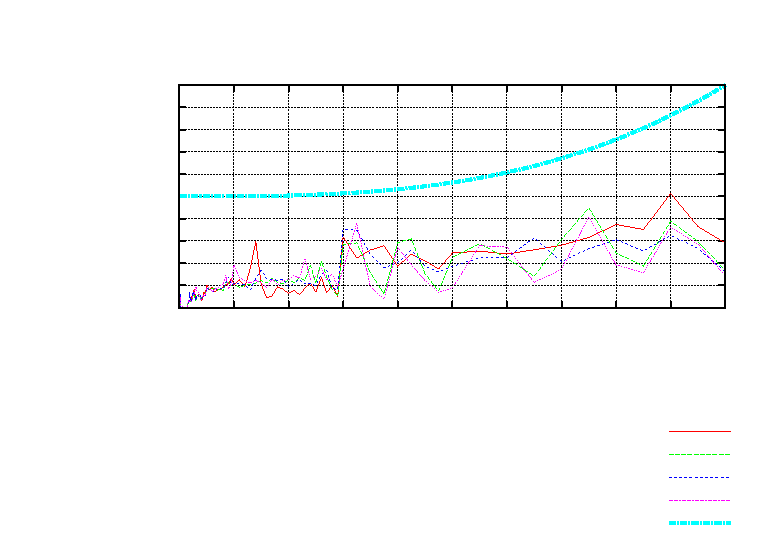
\includegraphics{ej3_nodos_n_star+bridge+double_star_sin_aspiracion_golosa}}%
    \gplfronttext
  \end{picture}%
\endgroup
}
    \caption{Complejidad temporal para grafos Estrella+Puente+Doble Estrella (Variante Max\_Iter=n),sin aspiraci\'on,golosa)}
\end{figure}

\begin{figure}[H]
    \centering
    \fontsize{8}{10}\selectfont
    \resizebox{0.8\textwidth}{!}{% GNUPLOT: LaTeX picture with Postscript
\begingroup
  \makeatletter
  \providecommand\color[2][]{%
    \GenericError{(gnuplot) \space\space\space\@spaces}{%
      Package color not loaded in conjunction with
      terminal option `colourtext'%
    }{See the gnuplot documentation for explanation.%
    }{Either use 'blacktext' in gnuplot or load the package
      color.sty in LaTeX.}%
    \renewcommand\color[2][]{}%
  }%
  \providecommand\includegraphics[2][]{%
    \GenericError{(gnuplot) \space\space\space\@spaces}{%
      Package graphicx or graphics not loaded%
    }{See the gnuplot documentation for explanation.%
    }{The gnuplot epslatex terminal needs graphicx.sty or graphics.sty.}%
    \renewcommand\includegraphics[2][]{}%
  }%
  \providecommand\rotatebox[2]{#2}%
  \@ifundefined{ifGPcolor}{%
    \newif\ifGPcolor
    \GPcolortrue
  }{}%
  \@ifundefined{ifGPblacktext}{%
    \newif\ifGPblacktext
    \GPblacktexttrue
  }{}%
  % define a \g@addto@macro without @ in the name:
  \let\gplgaddtomacro\g@addto@macro
  % define empty templates for all commands taking text:
  \gdef\gplbacktext{}%
  \gdef\gplfronttext{}%
  \makeatother
  \ifGPblacktext
    % no textcolor at all
    \def\colorrgb#1{}%
    \def\colorgray#1{}%
  \else
    % gray or color?
    \ifGPcolor
      \def\colorrgb#1{\color[rgb]{#1}}%
      \def\colorgray#1{\color[gray]{#1}}%
      \expandafter\def\csname LTw\endcsname{\color{white}}%
      \expandafter\def\csname LTb\endcsname{\color{black}}%
      \expandafter\def\csname LTa\endcsname{\color{black}}%
      \expandafter\def\csname LT0\endcsname{\color[rgb]{1,0,0}}%
      \expandafter\def\csname LT1\endcsname{\color[rgb]{0,1,0}}%
      \expandafter\def\csname LT2\endcsname{\color[rgb]{0,0,1}}%
      \expandafter\def\csname LT3\endcsname{\color[rgb]{1,0,1}}%
      \expandafter\def\csname LT4\endcsname{\color[rgb]{0,1,1}}%
      \expandafter\def\csname LT5\endcsname{\color[rgb]{1,1,0}}%
      \expandafter\def\csname LT6\endcsname{\color[rgb]{0,0,0}}%
      \expandafter\def\csname LT7\endcsname{\color[rgb]{1,0.3,0}}%
      \expandafter\def\csname LT8\endcsname{\color[rgb]{0.5,0.5,0.5}}%
    \else
      % gray
      \def\colorrgb#1{\color{black}}%
      \def\colorgray#1{\color[gray]{#1}}%
      \expandafter\def\csname LTw\endcsname{\color{white}}%
      \expandafter\def\csname LTb\endcsname{\color{black}}%
      \expandafter\def\csname LTa\endcsname{\color{black}}%
      \expandafter\def\csname LT0\endcsname{\color{black}}%
      \expandafter\def\csname LT1\endcsname{\color{black}}%
      \expandafter\def\csname LT2\endcsname{\color{black}}%
      \expandafter\def\csname LT3\endcsname{\color{black}}%
      \expandafter\def\csname LT4\endcsname{\color{black}}%
      \expandafter\def\csname LT5\endcsname{\color{black}}%
      \expandafter\def\csname LT6\endcsname{\color{black}}%
      \expandafter\def\csname LT7\endcsname{\color{black}}%
      \expandafter\def\csname LT8\endcsname{\color{black}}%
    \fi
  \fi
  \setlength{\unitlength}{0.0500bp}%
  \begin{picture}(7200.00,5040.00)%
    \gplgaddtomacro\gplbacktext{%
      \csname LTb\endcsname%
      \put(1034,3124){\makebox(0,0)[r]{\strut{} 1}}%
      \csname LTb\endcsname%
      \put(1034,3263){\makebox(0,0)[r]{\strut{} 2}}%
      \csname LTb\endcsname%
      \put(1034,3403){\makebox(0,0)[r]{\strut{} 3}}%
      \csname LTb\endcsname%
      \put(1034,3542){\makebox(0,0)[r]{\strut{} 4}}%
      \csname LTb\endcsname%
      \put(1034,3682){\makebox(0,0)[r]{\strut{} 5}}%
      \csname LTb\endcsname%
      \put(1034,3821){\makebox(0,0)[r]{\strut{} 6}}%
      \csname LTb\endcsname%
      \put(1034,3961){\makebox(0,0)[r]{\strut{} 7}}%
      \csname LTb\endcsname%
      \put(1034,4100){\makebox(0,0)[r]{\strut{} 8}}%
      \csname LTb\endcsname%
      \put(1034,4240){\makebox(0,0)[r]{\strut{} 9}}%
      \csname LTb\endcsname%
      \put(1034,4379){\makebox(0,0)[r]{\strut{} 10}}%
      \csname LTb\endcsname%
      \put(1166,2904){\makebox(0,0){\strut{} 0}}%
      \csname LTb\endcsname%
      \put(1730,2904){\makebox(0,0){\strut{} 1000}}%
      \csname LTb\endcsname%
      \put(2293,2904){\makebox(0,0){\strut{} 2000}}%
      \csname LTb\endcsname%
      \put(2857,2904){\makebox(0,0){\strut{} 3000}}%
      \csname LTb\endcsname%
      \put(3421,2904){\makebox(0,0){\strut{} 4000}}%
      \csname LTb\endcsname%
      \put(3985,2904){\makebox(0,0){\strut{} 5000}}%
      \csname LTb\endcsname%
      \put(4548,2904){\makebox(0,0){\strut{} 6000}}%
      \csname LTb\endcsname%
      \put(5112,2904){\makebox(0,0){\strut{} 7000}}%
      \csname LTb\endcsname%
      \put(5676,2904){\makebox(0,0){\strut{} 8000}}%
      \csname LTb\endcsname%
      \put(6239,2904){\makebox(0,0){\strut{} 9000}}%
      \csname LTb\endcsname%
      \put(6803,2904){\makebox(0,0){\strut{} 10000}}%
      \put(176,3751){\rotatebox{-270}{\makebox(0,0){\strut{}Frontera}}}%
      \put(396,3751){\rotatebox{-270}{\makebox(0,0){\strut{}(Escala Lineal)}}}%
      \put(3984,2574){\makebox(0,0){\strut{}Cantidad de Nodos}}%
      \put(3984,2354){\makebox(0,0){\strut{}(Escala Lineal)}}%
      \put(3984,4709){\makebox(0,0){\strut{}Frontera obtenida segun cantidad de nodos}}%
    }%
    \gplgaddtomacro\gplfronttext{%
      \csname LTb\endcsname%
      \put(6329,1933){\makebox(0,0)[r]{\strut{}Iter=nlog(n),Sin Mejorar=n,Tiempo Tabu=n}}%
      \csname LTb\endcsname%
      \put(6329,1713){\makebox(0,0)[r]{\strut{}Iter=nlog(n),Sin Mejorar=n,Tiempo Tabu=n2}}%
      \csname LTb\endcsname%
      \put(6329,1493){\makebox(0,0)[r]{\strut{}Iter=nlog(n),Sin Mejorar=n2,Tiempo Tabu=n}}%
      \csname LTb\endcsname%
      \put(6329,1273){\makebox(0,0)[r]{\strut{}Iter=nlog(n),Sin Mejorar=n2,Tiempo Tabu=n2}}%
      \csname LTb\endcsname%
      \put(6329,1053){\makebox(0,0)[r]{\strut{}Iter=n,Sin Mejorar=n,Tiempo Tabu=n}}%
      \csname LTb\endcsname%
      \put(6329,833){\makebox(0,0)[r]{\strut{}Iter=n,Sin Mejorar=n,Tiempo Tabu=n2}}%
      \csname LTb\endcsname%
      \put(6329,613){\makebox(0,0)[r]{\strut{}Iter=n,Sin Mejorar=n2,Tiempo Tabu=n}}%
      \csname LTb\endcsname%
      \put(6329,393){\makebox(0,0)[r]{\strut{}Iter=n,Sin Mejorar=n2,Tiempo Tabu=n2}}%
      \csname LTb\endcsname%
      \put(6329,173){\makebox(0,0)[r]{\strut{}Solucion optima}}%
    }%
    \gplbacktext
    \put(0,0){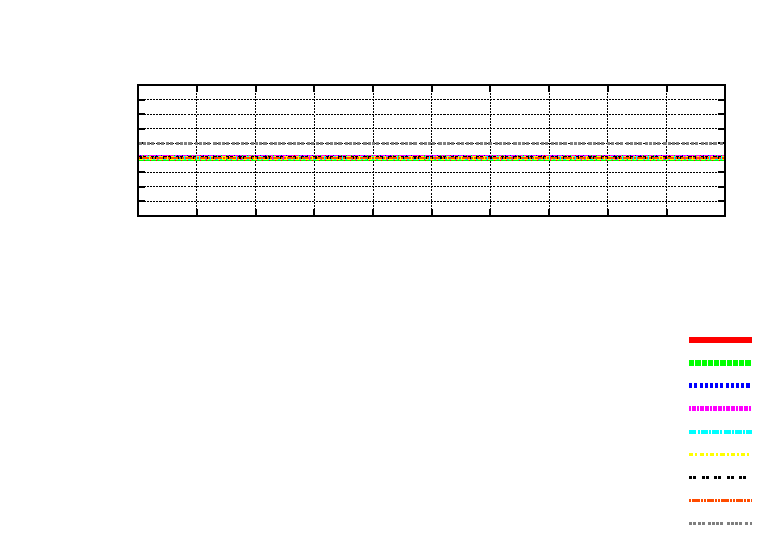
\includegraphics{ej3_frontera_star_bridge_double_star_sin_aspiracion_golosa}}%
    \gplfronttext
  \end{picture}%
\endgroup
}
    \caption{Frontera de grafos Estrella+Puente+Doble Estrella (sin aspiracion, golosa)}
\end{figure}

%Bipartito Completo
\begin{figure}[H]
    \centering
    \fontsize{8}{10}\selectfont
    \resizebox{0.8\textwidth}{!}{% GNUPLOT: LaTeX picture with Postscript
\begingroup
  \makeatletter
  \providecommand\color[2][]{%
    \GenericError{(gnuplot) \space\space\space\@spaces}{%
      Package color not loaded in conjunction with
      terminal option `colourtext'%
    }{See the gnuplot documentation for explanation.%
    }{Either use 'blacktext' in gnuplot or load the package
      color.sty in LaTeX.}%
    \renewcommand\color[2][]{}%
  }%
  \providecommand\includegraphics[2][]{%
    \GenericError{(gnuplot) \space\space\space\@spaces}{%
      Package graphicx or graphics not loaded%
    }{See the gnuplot documentation for explanation.%
    }{The gnuplot epslatex terminal needs graphicx.sty or graphics.sty.}%
    \renewcommand\includegraphics[2][]{}%
  }%
  \providecommand\rotatebox[2]{#2}%
  \@ifundefined{ifGPcolor}{%
    \newif\ifGPcolor
    \GPcolortrue
  }{}%
  \@ifundefined{ifGPblacktext}{%
    \newif\ifGPblacktext
    \GPblacktexttrue
  }{}%
  % define a \g@addto@macro without @ in the name:
  \let\gplgaddtomacro\g@addto@macro
  % define empty templates for all commands taking text:
  \gdef\gplbacktext{}%
  \gdef\gplfronttext{}%
  \makeatother
  \ifGPblacktext
    % no textcolor at all
    \def\colorrgb#1{}%
    \def\colorgray#1{}%
  \else
    % gray or color?
    \ifGPcolor
      \def\colorrgb#1{\color[rgb]{#1}}%
      \def\colorgray#1{\color[gray]{#1}}%
      \expandafter\def\csname LTw\endcsname{\color{white}}%
      \expandafter\def\csname LTb\endcsname{\color{black}}%
      \expandafter\def\csname LTa\endcsname{\color{black}}%
      \expandafter\def\csname LT0\endcsname{\color[rgb]{1,0,0}}%
      \expandafter\def\csname LT1\endcsname{\color[rgb]{0,1,0}}%
      \expandafter\def\csname LT2\endcsname{\color[rgb]{0,0,1}}%
      \expandafter\def\csname LT3\endcsname{\color[rgb]{1,0,1}}%
      \expandafter\def\csname LT4\endcsname{\color[rgb]{0,1,1}}%
      \expandafter\def\csname LT5\endcsname{\color[rgb]{1,1,0}}%
      \expandafter\def\csname LT6\endcsname{\color[rgb]{0,0,0}}%
      \expandafter\def\csname LT7\endcsname{\color[rgb]{1,0.3,0}}%
      \expandafter\def\csname LT8\endcsname{\color[rgb]{0.5,0.5,0.5}}%
    \else
      % gray
      \def\colorrgb#1{\color{black}}%
      \def\colorgray#1{\color[gray]{#1}}%
      \expandafter\def\csname LTw\endcsname{\color{white}}%
      \expandafter\def\csname LTb\endcsname{\color{black}}%
      \expandafter\def\csname LTa\endcsname{\color{black}}%
      \expandafter\def\csname LT0\endcsname{\color{black}}%
      \expandafter\def\csname LT1\endcsname{\color{black}}%
      \expandafter\def\csname LT2\endcsname{\color{black}}%
      \expandafter\def\csname LT3\endcsname{\color{black}}%
      \expandafter\def\csname LT4\endcsname{\color{black}}%
      \expandafter\def\csname LT5\endcsname{\color{black}}%
      \expandafter\def\csname LT6\endcsname{\color{black}}%
      \expandafter\def\csname LT7\endcsname{\color{black}}%
      \expandafter\def\csname LT8\endcsname{\color{black}}%
    \fi
  \fi
  \setlength{\unitlength}{0.0500bp}%
  \begin{picture}(7200.00,5040.00)%
    \gplgaddtomacro\gplbacktext{%
      \csname LTb\endcsname%
      \put(1694,2244){\makebox(0,0)[r]{\strut{} 0}}%
      \csname LTb\endcsname%
      \put(1694,2671){\makebox(0,0)[r]{\strut{} 5e+06}}%
      \csname LTb\endcsname%
      \put(1694,3098){\makebox(0,0)[r]{\strut{} 1e+07}}%
      \csname LTb\endcsname%
      \put(1694,3525){\makebox(0,0)[r]{\strut{} 1.5e+07}}%
      \csname LTb\endcsname%
      \put(1694,3952){\makebox(0,0)[r]{\strut{} 2e+07}}%
      \csname LTb\endcsname%
      \put(1694,4379){\makebox(0,0)[r]{\strut{} 2.5e+07}}%
      \csname LTb\endcsname%
      \put(1826,2024){\makebox(0,0){\strut{} 0}}%
      \csname LTb\endcsname%
      \put(2324,2024){\makebox(0,0){\strut{} 500}}%
      \csname LTb\endcsname%
      \put(2821,2024){\makebox(0,0){\strut{} 1000}}%
      \csname LTb\endcsname%
      \put(3319,2024){\makebox(0,0){\strut{} 1500}}%
      \csname LTb\endcsname%
      \put(3817,2024){\makebox(0,0){\strut{} 2000}}%
      \csname LTb\endcsname%
      \put(4315,2024){\makebox(0,0){\strut{} 2500}}%
      \csname LTb\endcsname%
      \put(4812,2024){\makebox(0,0){\strut{} 3000}}%
      \csname LTb\endcsname%
      \put(5310,2024){\makebox(0,0){\strut{} 3500}}%
      \csname LTb\endcsname%
      \put(5808,2024){\makebox(0,0){\strut{} 4000}}%
      \csname LTb\endcsname%
      \put(6305,2024){\makebox(0,0){\strut{} 4500}}%
      \csname LTb\endcsname%
      \put(6803,2024){\makebox(0,0){\strut{} 5000}}%
      \put(176,3311){\rotatebox{-270}{\makebox(0,0){\strut{}Tiempo (microsegundos)}}}%
      \put(396,3311){\rotatebox{-270}{\makebox(0,0){\strut{}(Escala Lineal)}}}%
      \put(4314,1694){\makebox(0,0){\strut{}Cantidad de Nodos}}%
      \put(4314,1474){\makebox(0,0){\strut{}(Escala Lineal)}}%
      \put(4314,4709){\makebox(0,0){\strut{}Tiempo de ejecucion conforme aumenta la cantidad de nodos}}%
    }%
    \gplgaddtomacro\gplfronttext{%
      \csname LTb\endcsname%
      \put(6659,1053){\makebox(0,0)[r]{\strut{}Iter=nlog(n),Sin Mejorar=n,Tiempo Tabu=n}}%
      \csname LTb\endcsname%
      \put(6659,833){\makebox(0,0)[r]{\strut{}Iter=nlog(n),Sin Mejorar=n,Tiempo Tabu=n2}}%
      \csname LTb\endcsname%
      \put(6659,613){\makebox(0,0)[r]{\strut{}Iter=nlog(n),Sin Mejorar=n2,Tiempo Tabu=n}}%
      \csname LTb\endcsname%
      \put(6659,393){\makebox(0,0)[r]{\strut{}Iter=nlog(n),Sin Mejorar=n2,Tiempo Tabu=n2}}%
      \csname LTb\endcsname%
      \put(6659,173){\makebox(0,0)[r]{\strut{}Cota teórica superior $\mathcal O(n^3 \cdot log(n))$}}%
    }%
    \gplbacktext
    \put(0,0){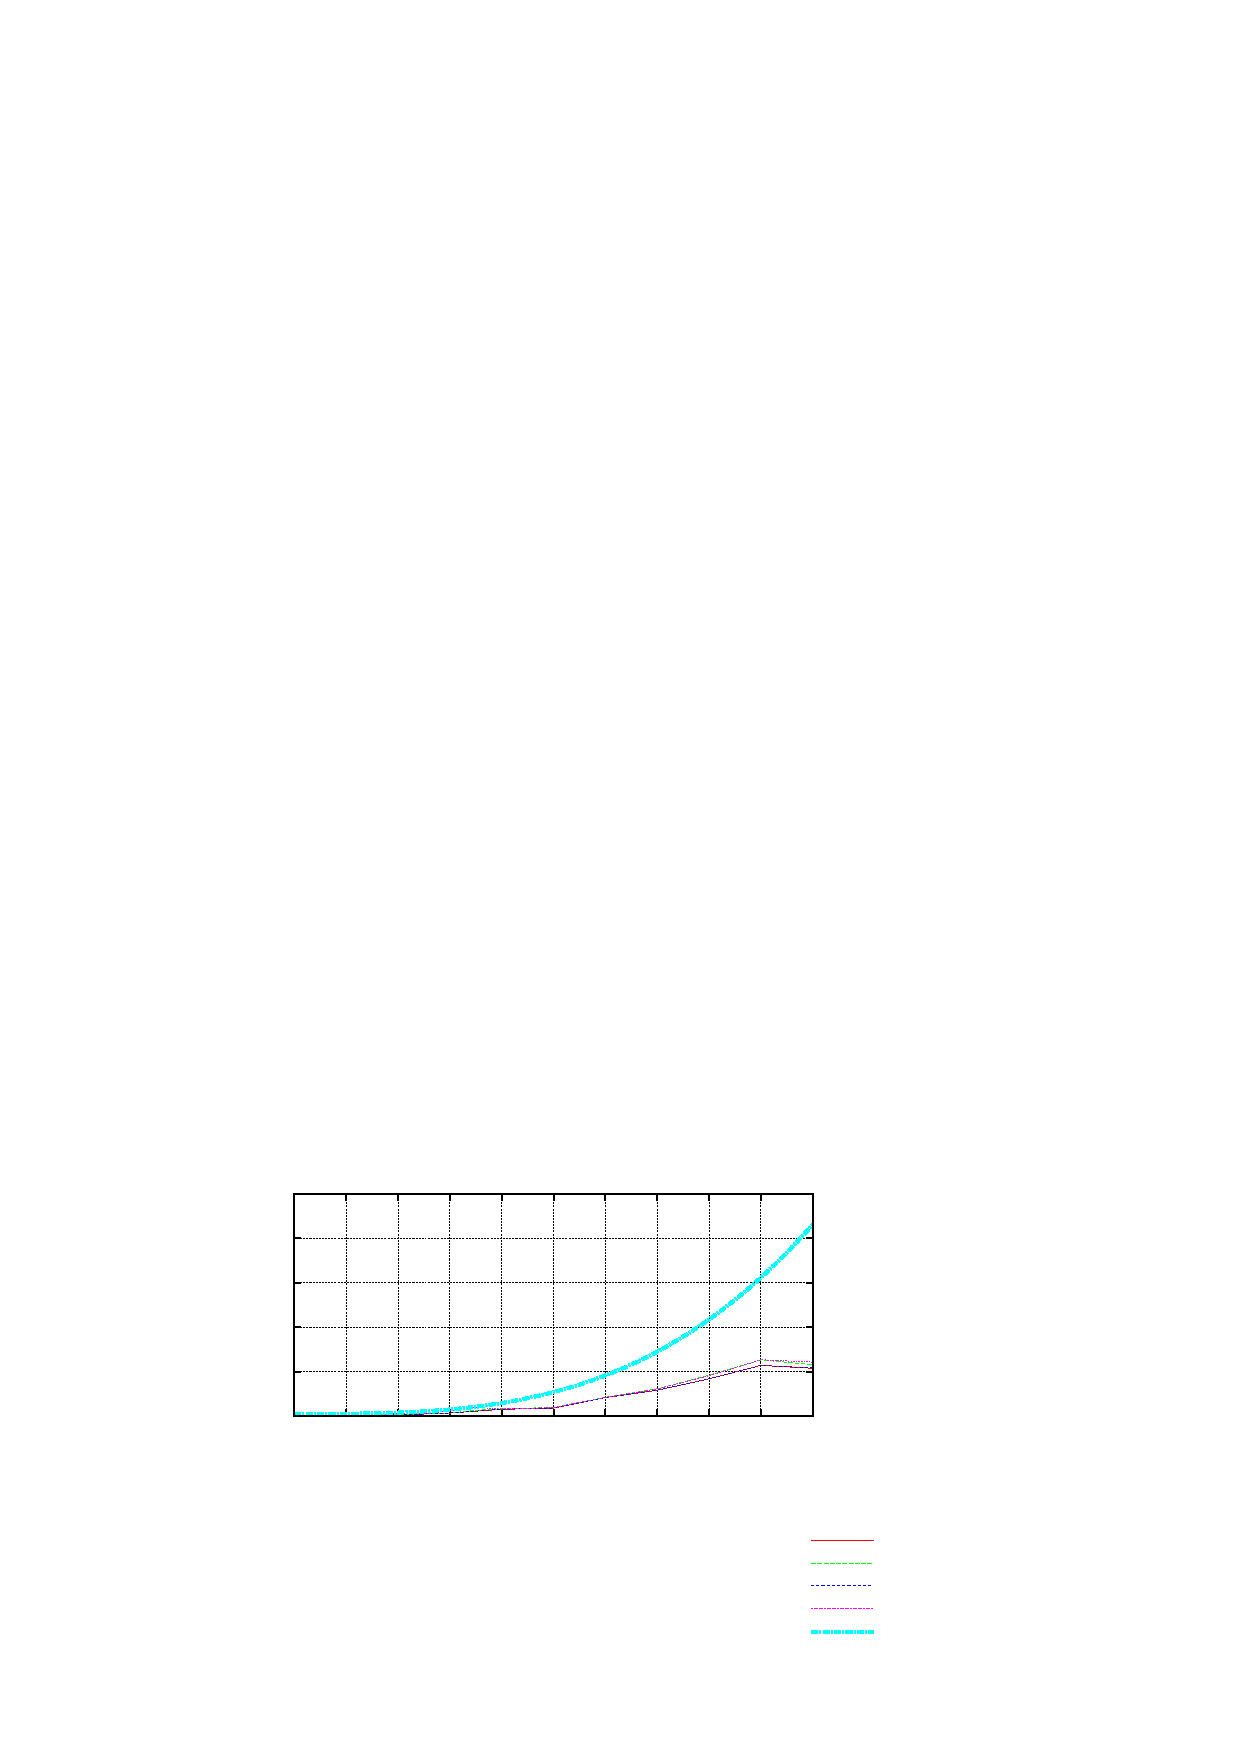
\includegraphics{ej3_nodos_nlogn_complete_bipartite}}%
    \gplfronttext
  \end{picture}%
\endgroup
}
    \caption{Complejidad temporal para grafos Bipartito Completo (Variante Max\_Iter=nlog(n))}
\end{figure}

\begin{figure}[H]
    \centering
    \fontsize{8}{10}\selectfont
    \resizebox{0.8\textwidth}{!}{% GNUPLOT: LaTeX picture with Postscript
\begingroup
  \makeatletter
  \providecommand\color[2][]{%
    \GenericError{(gnuplot) \space\space\space\@spaces}{%
      Package color not loaded in conjunction with
      terminal option `colourtext'%
    }{See the gnuplot documentation for explanation.%
    }{Either use 'blacktext' in gnuplot or load the package
      color.sty in LaTeX.}%
    \renewcommand\color[2][]{}%
  }%
  \providecommand\includegraphics[2][]{%
    \GenericError{(gnuplot) \space\space\space\@spaces}{%
      Package graphicx or graphics not loaded%
    }{See the gnuplot documentation for explanation.%
    }{The gnuplot epslatex terminal needs graphicx.sty or graphics.sty.}%
    \renewcommand\includegraphics[2][]{}%
  }%
  \providecommand\rotatebox[2]{#2}%
  \@ifundefined{ifGPcolor}{%
    \newif\ifGPcolor
    \GPcolortrue
  }{}%
  \@ifundefined{ifGPblacktext}{%
    \newif\ifGPblacktext
    \GPblacktexttrue
  }{}%
  % define a \g@addto@macro without @ in the name:
  \let\gplgaddtomacro\g@addto@macro
  % define empty templates for all commands taking text:
  \gdef\gplbacktext{}%
  \gdef\gplfronttext{}%
  \makeatother
  \ifGPblacktext
    % no textcolor at all
    \def\colorrgb#1{}%
    \def\colorgray#1{}%
  \else
    % gray or color?
    \ifGPcolor
      \def\colorrgb#1{\color[rgb]{#1}}%
      \def\colorgray#1{\color[gray]{#1}}%
      \expandafter\def\csname LTw\endcsname{\color{white}}%
      \expandafter\def\csname LTb\endcsname{\color{black}}%
      \expandafter\def\csname LTa\endcsname{\color{black}}%
      \expandafter\def\csname LT0\endcsname{\color[rgb]{1,0,0}}%
      \expandafter\def\csname LT1\endcsname{\color[rgb]{0,1,0}}%
      \expandafter\def\csname LT2\endcsname{\color[rgb]{0,0,1}}%
      \expandafter\def\csname LT3\endcsname{\color[rgb]{1,0,1}}%
      \expandafter\def\csname LT4\endcsname{\color[rgb]{0,1,1}}%
      \expandafter\def\csname LT5\endcsname{\color[rgb]{1,1,0}}%
      \expandafter\def\csname LT6\endcsname{\color[rgb]{0,0,0}}%
      \expandafter\def\csname LT7\endcsname{\color[rgb]{1,0.3,0}}%
      \expandafter\def\csname LT8\endcsname{\color[rgb]{0.5,0.5,0.5}}%
    \else
      % gray
      \def\colorrgb#1{\color{black}}%
      \def\colorgray#1{\color[gray]{#1}}%
      \expandafter\def\csname LTw\endcsname{\color{white}}%
      \expandafter\def\csname LTb\endcsname{\color{black}}%
      \expandafter\def\csname LTa\endcsname{\color{black}}%
      \expandafter\def\csname LT0\endcsname{\color{black}}%
      \expandafter\def\csname LT1\endcsname{\color{black}}%
      \expandafter\def\csname LT2\endcsname{\color{black}}%
      \expandafter\def\csname LT3\endcsname{\color{black}}%
      \expandafter\def\csname LT4\endcsname{\color{black}}%
      \expandafter\def\csname LT5\endcsname{\color{black}}%
      \expandafter\def\csname LT6\endcsname{\color{black}}%
      \expandafter\def\csname LT7\endcsname{\color{black}}%
      \expandafter\def\csname LT8\endcsname{\color{black}}%
    \fi
  \fi
  \setlength{\unitlength}{0.0500bp}%
  \begin{picture}(7200.00,5040.00)%
    \gplgaddtomacro\gplbacktext{%
      \csname LTb\endcsname%
      \put(1694,2244){\makebox(0,0)[r]{\strut{} 0}}%
      \csname LTb\endcsname%
      \put(1694,2511){\makebox(0,0)[r]{\strut{} 200000}}%
      \csname LTb\endcsname%
      \put(1694,2778){\makebox(0,0)[r]{\strut{} 400000}}%
      \csname LTb\endcsname%
      \put(1694,3045){\makebox(0,0)[r]{\strut{} 600000}}%
      \csname LTb\endcsname%
      \put(1694,3312){\makebox(0,0)[r]{\strut{} 800000}}%
      \csname LTb\endcsname%
      \put(1694,3578){\makebox(0,0)[r]{\strut{} 1e+06}}%
      \csname LTb\endcsname%
      \put(1694,3845){\makebox(0,0)[r]{\strut{} 1.2e+06}}%
      \csname LTb\endcsname%
      \put(1694,4112){\makebox(0,0)[r]{\strut{} 1.4e+06}}%
      \csname LTb\endcsname%
      \put(1694,4379){\makebox(0,0)[r]{\strut{} 1.6e+06}}%
      \csname LTb\endcsname%
      \put(1826,2024){\makebox(0,0){\strut{} 0}}%
      \csname LTb\endcsname%
      \put(2324,2024){\makebox(0,0){\strut{} 500}}%
      \csname LTb\endcsname%
      \put(2821,2024){\makebox(0,0){\strut{} 1000}}%
      \csname LTb\endcsname%
      \put(3319,2024){\makebox(0,0){\strut{} 1500}}%
      \csname LTb\endcsname%
      \put(3817,2024){\makebox(0,0){\strut{} 2000}}%
      \csname LTb\endcsname%
      \put(4315,2024){\makebox(0,0){\strut{} 2500}}%
      \csname LTb\endcsname%
      \put(4812,2024){\makebox(0,0){\strut{} 3000}}%
      \csname LTb\endcsname%
      \put(5310,2024){\makebox(0,0){\strut{} 3500}}%
      \csname LTb\endcsname%
      \put(5808,2024){\makebox(0,0){\strut{} 4000}}%
      \csname LTb\endcsname%
      \put(6305,2024){\makebox(0,0){\strut{} 4500}}%
      \csname LTb\endcsname%
      \put(6803,2024){\makebox(0,0){\strut{} 5000}}%
      \put(176,3311){\rotatebox{-270}{\makebox(0,0){\strut{}Tiempo (microsegundos)}}}%
      \put(396,3311){\rotatebox{-270}{\makebox(0,0){\strut{}(Escala Lineal)}}}%
      \put(4314,1694){\makebox(0,0){\strut{}Cantidad de Nodos}}%
      \put(4314,1474){\makebox(0,0){\strut{}(Escala Lineal)}}%
      \put(4314,4709){\makebox(0,0){\strut{}Tiempo de ejecucion conforme aumenta la cantidad de nodos}}%
    }%
    \gplgaddtomacro\gplfronttext{%
      \csname LTb\endcsname%
      \put(6263,1053){\makebox(0,0)[r]{\strut{}Iter=n,Sin Mejorar=n,Tiempo Tabu=n}}%
      \csname LTb\endcsname%
      \put(6263,833){\makebox(0,0)[r]{\strut{}Iter=n,Sin Mejorar=n,Tiempo Tabu=n2}}%
      \csname LTb\endcsname%
      \put(6263,613){\makebox(0,0)[r]{\strut{}Iter=n,Sin Mejorar=n2,Tiempo Tabu=n}}%
      \csname LTb\endcsname%
      \put(6263,393){\makebox(0,0)[r]{\strut{}Iter=n,Sin Mejorar=n2,Tiempo Tabu=n2}}%
      \csname LTb\endcsname%
      \put(6263,173){\makebox(0,0)[r]{\strut{}Cota teórica superior $\mathcal O(n^3)$}}%
    }%
    \gplbacktext
    \put(0,0){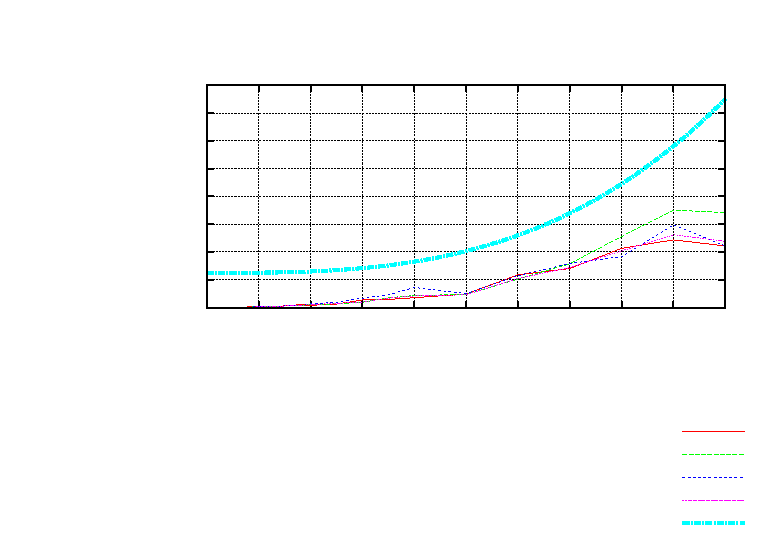
\includegraphics{ej3_nodos_n_complete_bipartite}}%
    \gplfronttext
  \end{picture}%
\endgroup
}
    \caption{Complejidad temporal para grafos Bipartito Completo (Variante Max\_Iter=n)}
\end{figure}

\begin{figure}[H]
    \centering
    \fontsize{8}{10}\selectfont
    \resizebox{0.8\textwidth}{!}{% GNUPLOT: LaTeX picture with Postscript
\begingroup
  \makeatletter
  \providecommand\color[2][]{%
    \GenericError{(gnuplot) \space\space\space\@spaces}{%
      Package color not loaded in conjunction with
      terminal option `colourtext'%
    }{See the gnuplot documentation for explanation.%
    }{Either use 'blacktext' in gnuplot or load the package
      color.sty in LaTeX.}%
    \renewcommand\color[2][]{}%
  }%
  \providecommand\includegraphics[2][]{%
    \GenericError{(gnuplot) \space\space\space\@spaces}{%
      Package graphicx or graphics not loaded%
    }{See the gnuplot documentation for explanation.%
    }{The gnuplot epslatex terminal needs graphicx.sty or graphics.sty.}%
    \renewcommand\includegraphics[2][]{}%
  }%
  \providecommand\rotatebox[2]{#2}%
  \@ifundefined{ifGPcolor}{%
    \newif\ifGPcolor
    \GPcolortrue
  }{}%
  \@ifundefined{ifGPblacktext}{%
    \newif\ifGPblacktext
    \GPblacktexttrue
  }{}%
  % define a \g@addto@macro without @ in the name:
  \let\gplgaddtomacro\g@addto@macro
  % define empty templates for all commands taking text:
  \gdef\gplbacktext{}%
  \gdef\gplfronttext{}%
  \makeatother
  \ifGPblacktext
    % no textcolor at all
    \def\colorrgb#1{}%
    \def\colorgray#1{}%
  \else
    % gray or color?
    \ifGPcolor
      \def\colorrgb#1{\color[rgb]{#1}}%
      \def\colorgray#1{\color[gray]{#1}}%
      \expandafter\def\csname LTw\endcsname{\color{white}}%
      \expandafter\def\csname LTb\endcsname{\color{black}}%
      \expandafter\def\csname LTa\endcsname{\color{black}}%
      \expandafter\def\csname LT0\endcsname{\color[rgb]{1,0,0}}%
      \expandafter\def\csname LT1\endcsname{\color[rgb]{0,1,0}}%
      \expandafter\def\csname LT2\endcsname{\color[rgb]{0,0,1}}%
      \expandafter\def\csname LT3\endcsname{\color[rgb]{1,0,1}}%
      \expandafter\def\csname LT4\endcsname{\color[rgb]{0,1,1}}%
      \expandafter\def\csname LT5\endcsname{\color[rgb]{1,1,0}}%
      \expandafter\def\csname LT6\endcsname{\color[rgb]{0,0,0}}%
      \expandafter\def\csname LT7\endcsname{\color[rgb]{1,0.3,0}}%
      \expandafter\def\csname LT8\endcsname{\color[rgb]{0.5,0.5,0.5}}%
    \else
      % gray
      \def\colorrgb#1{\color{black}}%
      \def\colorgray#1{\color[gray]{#1}}%
      \expandafter\def\csname LTw\endcsname{\color{white}}%
      \expandafter\def\csname LTb\endcsname{\color{black}}%
      \expandafter\def\csname LTa\endcsname{\color{black}}%
      \expandafter\def\csname LT0\endcsname{\color{black}}%
      \expandafter\def\csname LT1\endcsname{\color{black}}%
      \expandafter\def\csname LT2\endcsname{\color{black}}%
      \expandafter\def\csname LT3\endcsname{\color{black}}%
      \expandafter\def\csname LT4\endcsname{\color{black}}%
      \expandafter\def\csname LT5\endcsname{\color{black}}%
      \expandafter\def\csname LT6\endcsname{\color{black}}%
      \expandafter\def\csname LT7\endcsname{\color{black}}%
      \expandafter\def\csname LT8\endcsname{\color{black}}%
    \fi
  \fi
  \setlength{\unitlength}{0.0500bp}%
  \begin{picture}(7200.00,5040.00)%
    \gplgaddtomacro\gplbacktext{%
      \csname LTb\endcsname%
      \put(1298,2904){\makebox(0,0)[r]{\strut{} 0}}%
      \csname LTb\endcsname%
      \put(1298,3052){\makebox(0,0)[r]{\strut{} 500}}%
      \csname LTb\endcsname%
      \put(1298,3199){\makebox(0,0)[r]{\strut{} 1000}}%
      \csname LTb\endcsname%
      \put(1298,3347){\makebox(0,0)[r]{\strut{} 1500}}%
      \csname LTb\endcsname%
      \put(1298,3494){\makebox(0,0)[r]{\strut{} 2000}}%
      \csname LTb\endcsname%
      \put(1298,3642){\makebox(0,0)[r]{\strut{} 2500}}%
      \csname LTb\endcsname%
      \put(1298,3789){\makebox(0,0)[r]{\strut{} 3000}}%
      \csname LTb\endcsname%
      \put(1298,3937){\makebox(0,0)[r]{\strut{} 3500}}%
      \csname LTb\endcsname%
      \put(1298,4084){\makebox(0,0)[r]{\strut{} 4000}}%
      \csname LTb\endcsname%
      \put(1298,4232){\makebox(0,0)[r]{\strut{} 4500}}%
      \csname LTb\endcsname%
      \put(1298,4379){\makebox(0,0)[r]{\strut{} 5000}}%
      \csname LTb\endcsname%
      \put(1430,2684){\makebox(0,0){\strut{} 0}}%
      \csname LTb\endcsname%
      \put(1967,2684){\makebox(0,0){\strut{} 500}}%
      \csname LTb\endcsname%
      \put(2505,2684){\makebox(0,0){\strut{} 1000}}%
      \csname LTb\endcsname%
      \put(3042,2684){\makebox(0,0){\strut{} 1500}}%
      \csname LTb\endcsname%
      \put(3579,2684){\makebox(0,0){\strut{} 2000}}%
      \csname LTb\endcsname%
      \put(4117,2684){\makebox(0,0){\strut{} 2500}}%
      \csname LTb\endcsname%
      \put(4654,2684){\makebox(0,0){\strut{} 3000}}%
      \csname LTb\endcsname%
      \put(5191,2684){\makebox(0,0){\strut{} 3500}}%
      \csname LTb\endcsname%
      \put(5728,2684){\makebox(0,0){\strut{} 4000}}%
      \csname LTb\endcsname%
      \put(6266,2684){\makebox(0,0){\strut{} 4500}}%
      \csname LTb\endcsname%
      \put(6803,2684){\makebox(0,0){\strut{} 5000}}%
      \put(176,3641){\rotatebox{-270}{\makebox(0,0){\strut{}Frontera}}}%
      \put(396,3641){\rotatebox{-270}{\makebox(0,0){\strut{}(Escala Lineal)}}}%
      \put(4116,2354){\makebox(0,0){\strut{}Cantidad de Nodos}}%
      \put(4116,2134){\makebox(0,0){\strut{}(Escala Lineal)}}%
      \put(4116,4709){\makebox(0,0){\strut{}Frontera obtenida segun cantidad de nodos}}%
    }%
    \gplgaddtomacro\gplfronttext{%
      \csname LTb\endcsname%
      \put(6461,1713){\makebox(0,0)[r]{\strut{}Iter=nlog(n),Sin Mejorar=n,Tiempo Tabu=n}}%
      \csname LTb\endcsname%
      \put(6461,1493){\makebox(0,0)[r]{\strut{}Iter=nlog(n),Sin Mejorar=n,Tiempo Tabu=n2}}%
      \csname LTb\endcsname%
      \put(6461,1273){\makebox(0,0)[r]{\strut{}Iter=nlog(n),Sin Mejorar=n2,Tiempo Tabu=n}}%
      \csname LTb\endcsname%
      \put(6461,1053){\makebox(0,0)[r]{\strut{}Iter=nlog(n),Sin Mejorar=n2,Tiempo Tabu=n2}}%
      \csname LTb\endcsname%
      \put(6461,833){\makebox(0,0)[r]{\strut{}Iter=n,Sin Mejorar=n,Tiempo Tabu=n}}%
      \csname LTb\endcsname%
      \put(6461,613){\makebox(0,0)[r]{\strut{}Iter=n,Sin Mejorar=n,Tiempo Tabu=n2}}%
      \csname LTb\endcsname%
      \put(6461,393){\makebox(0,0)[r]{\strut{}Iter=n,Sin Mejorar=n2,Tiempo Tabu=n}}%
      \csname LTb\endcsname%
      \put(6461,173){\makebox(0,0)[r]{\strut{}Iter=n,Sin Mejorar=n2,Tiempo Tabu=n2}}%
    }%
    \gplbacktext
    \put(0,0){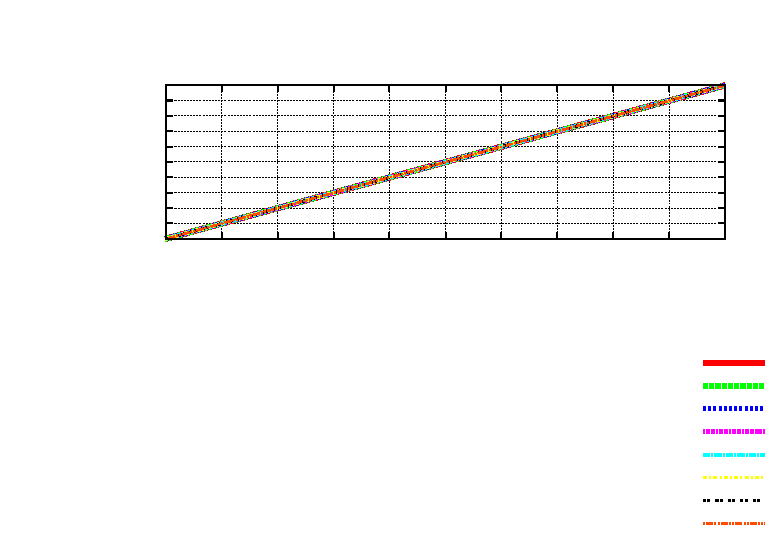
\includegraphics{ej3_frontera_complete_bipartite}}%
    \gplfronttext
  \end{picture}%
\endgroup
}
    \caption{Frontera de grafos Bipartito Completo}
\end{figure}

%Bipartito Completo sin aspiracion
\begin{figure}[H]
    \centering
    \fontsize{8}{10}\selectfont
    \resizebox{0.8\textwidth}{!}{% GNUPLOT: LaTeX picture with Postscript
\begingroup
  \makeatletter
  \providecommand\color[2][]{%
    \GenericError{(gnuplot) \space\space\space\@spaces}{%
      Package color not loaded in conjunction with
      terminal option `colourtext'%
    }{See the gnuplot documentation for explanation.%
    }{Either use 'blacktext' in gnuplot or load the package
      color.sty in LaTeX.}%
    \renewcommand\color[2][]{}%
  }%
  \providecommand\includegraphics[2][]{%
    \GenericError{(gnuplot) \space\space\space\@spaces}{%
      Package graphicx or graphics not loaded%
    }{See the gnuplot documentation for explanation.%
    }{The gnuplot epslatex terminal needs graphicx.sty or graphics.sty.}%
    \renewcommand\includegraphics[2][]{}%
  }%
  \providecommand\rotatebox[2]{#2}%
  \@ifundefined{ifGPcolor}{%
    \newif\ifGPcolor
    \GPcolortrue
  }{}%
  \@ifundefined{ifGPblacktext}{%
    \newif\ifGPblacktext
    \GPblacktexttrue
  }{}%
  % define a \g@addto@macro without @ in the name:
  \let\gplgaddtomacro\g@addto@macro
  % define empty templates for all commands taking text:
  \gdef\gplbacktext{}%
  \gdef\gplfronttext{}%
  \makeatother
  \ifGPblacktext
    % no textcolor at all
    \def\colorrgb#1{}%
    \def\colorgray#1{}%
  \else
    % gray or color?
    \ifGPcolor
      \def\colorrgb#1{\color[rgb]{#1}}%
      \def\colorgray#1{\color[gray]{#1}}%
      \expandafter\def\csname LTw\endcsname{\color{white}}%
      \expandafter\def\csname LTb\endcsname{\color{black}}%
      \expandafter\def\csname LTa\endcsname{\color{black}}%
      \expandafter\def\csname LT0\endcsname{\color[rgb]{1,0,0}}%
      \expandafter\def\csname LT1\endcsname{\color[rgb]{0,1,0}}%
      \expandafter\def\csname LT2\endcsname{\color[rgb]{0,0,1}}%
      \expandafter\def\csname LT3\endcsname{\color[rgb]{1,0,1}}%
      \expandafter\def\csname LT4\endcsname{\color[rgb]{0,1,1}}%
      \expandafter\def\csname LT5\endcsname{\color[rgb]{1,1,0}}%
      \expandafter\def\csname LT6\endcsname{\color[rgb]{0,0,0}}%
      \expandafter\def\csname LT7\endcsname{\color[rgb]{1,0.3,0}}%
      \expandafter\def\csname LT8\endcsname{\color[rgb]{0.5,0.5,0.5}}%
    \else
      % gray
      \def\colorrgb#1{\color{black}}%
      \def\colorgray#1{\color[gray]{#1}}%
      \expandafter\def\csname LTw\endcsname{\color{white}}%
      \expandafter\def\csname LTb\endcsname{\color{black}}%
      \expandafter\def\csname LTa\endcsname{\color{black}}%
      \expandafter\def\csname LT0\endcsname{\color{black}}%
      \expandafter\def\csname LT1\endcsname{\color{black}}%
      \expandafter\def\csname LT2\endcsname{\color{black}}%
      \expandafter\def\csname LT3\endcsname{\color{black}}%
      \expandafter\def\csname LT4\endcsname{\color{black}}%
      \expandafter\def\csname LT5\endcsname{\color{black}}%
      \expandafter\def\csname LT6\endcsname{\color{black}}%
      \expandafter\def\csname LT7\endcsname{\color{black}}%
      \expandafter\def\csname LT8\endcsname{\color{black}}%
    \fi
  \fi
  \setlength{\unitlength}{0.0500bp}%
  \begin{picture}(7200.00,5040.00)%
    \gplgaddtomacro\gplbacktext{%
      \csname LTb\endcsname%
      \put(1694,2244){\makebox(0,0)[r]{\strut{} 0}}%
      \csname LTb\endcsname%
      \put(1694,2671){\makebox(0,0)[r]{\strut{} 5e+06}}%
      \csname LTb\endcsname%
      \put(1694,3098){\makebox(0,0)[r]{\strut{} 1e+07}}%
      \csname LTb\endcsname%
      \put(1694,3525){\makebox(0,0)[r]{\strut{} 1.5e+07}}%
      \csname LTb\endcsname%
      \put(1694,3952){\makebox(0,0)[r]{\strut{} 2e+07}}%
      \csname LTb\endcsname%
      \put(1694,4379){\makebox(0,0)[r]{\strut{} 2.5e+07}}%
      \csname LTb\endcsname%
      \put(1826,2024){\makebox(0,0){\strut{} 0}}%
      \csname LTb\endcsname%
      \put(2324,2024){\makebox(0,0){\strut{} 500}}%
      \csname LTb\endcsname%
      \put(2821,2024){\makebox(0,0){\strut{} 1000}}%
      \csname LTb\endcsname%
      \put(3319,2024){\makebox(0,0){\strut{} 1500}}%
      \csname LTb\endcsname%
      \put(3817,2024){\makebox(0,0){\strut{} 2000}}%
      \csname LTb\endcsname%
      \put(4315,2024){\makebox(0,0){\strut{} 2500}}%
      \csname LTb\endcsname%
      \put(4812,2024){\makebox(0,0){\strut{} 3000}}%
      \csname LTb\endcsname%
      \put(5310,2024){\makebox(0,0){\strut{} 3500}}%
      \csname LTb\endcsname%
      \put(5808,2024){\makebox(0,0){\strut{} 4000}}%
      \csname LTb\endcsname%
      \put(6305,2024){\makebox(0,0){\strut{} 4500}}%
      \csname LTb\endcsname%
      \put(6803,2024){\makebox(0,0){\strut{} 5000}}%
      \put(176,3311){\rotatebox{-270}{\makebox(0,0){\strut{}Tiempo (microsegundos)}}}%
      \put(396,3311){\rotatebox{-270}{\makebox(0,0){\strut{}(Escala Lineal)}}}%
      \put(4314,1694){\makebox(0,0){\strut{}Cantidad de Nodos}}%
      \put(4314,1474){\makebox(0,0){\strut{}(Escala Lineal)}}%
      \put(4314,4709){\makebox(0,0){\strut{}Tiempo de ejecucion conforme aumenta la cantidad de nodos}}%
    }%
    \gplgaddtomacro\gplfronttext{%
      \csname LTb\endcsname%
      \put(6659,1053){\makebox(0,0)[r]{\strut{}Iter=nlog(n),Sin Mejorar=n,Tiempo Tabu=n}}%
      \csname LTb\endcsname%
      \put(6659,833){\makebox(0,0)[r]{\strut{}Iter=nlog(n),Sin Mejorar=n,Tiempo Tabu=n2}}%
      \csname LTb\endcsname%
      \put(6659,613){\makebox(0,0)[r]{\strut{}Iter=nlog(n),Sin Mejorar=n2,Tiempo Tabu=n}}%
      \csname LTb\endcsname%
      \put(6659,393){\makebox(0,0)[r]{\strut{}Iter=nlog(n),Sin Mejorar=n2,Tiempo Tabu=n2}}%
      \csname LTb\endcsname%
      \put(6659,173){\makebox(0,0)[r]{\strut{}Cota teórica superior $\mathcal O(n^3 \cdot log(n))$}}%
    }%
    \gplbacktext
    \put(0,0){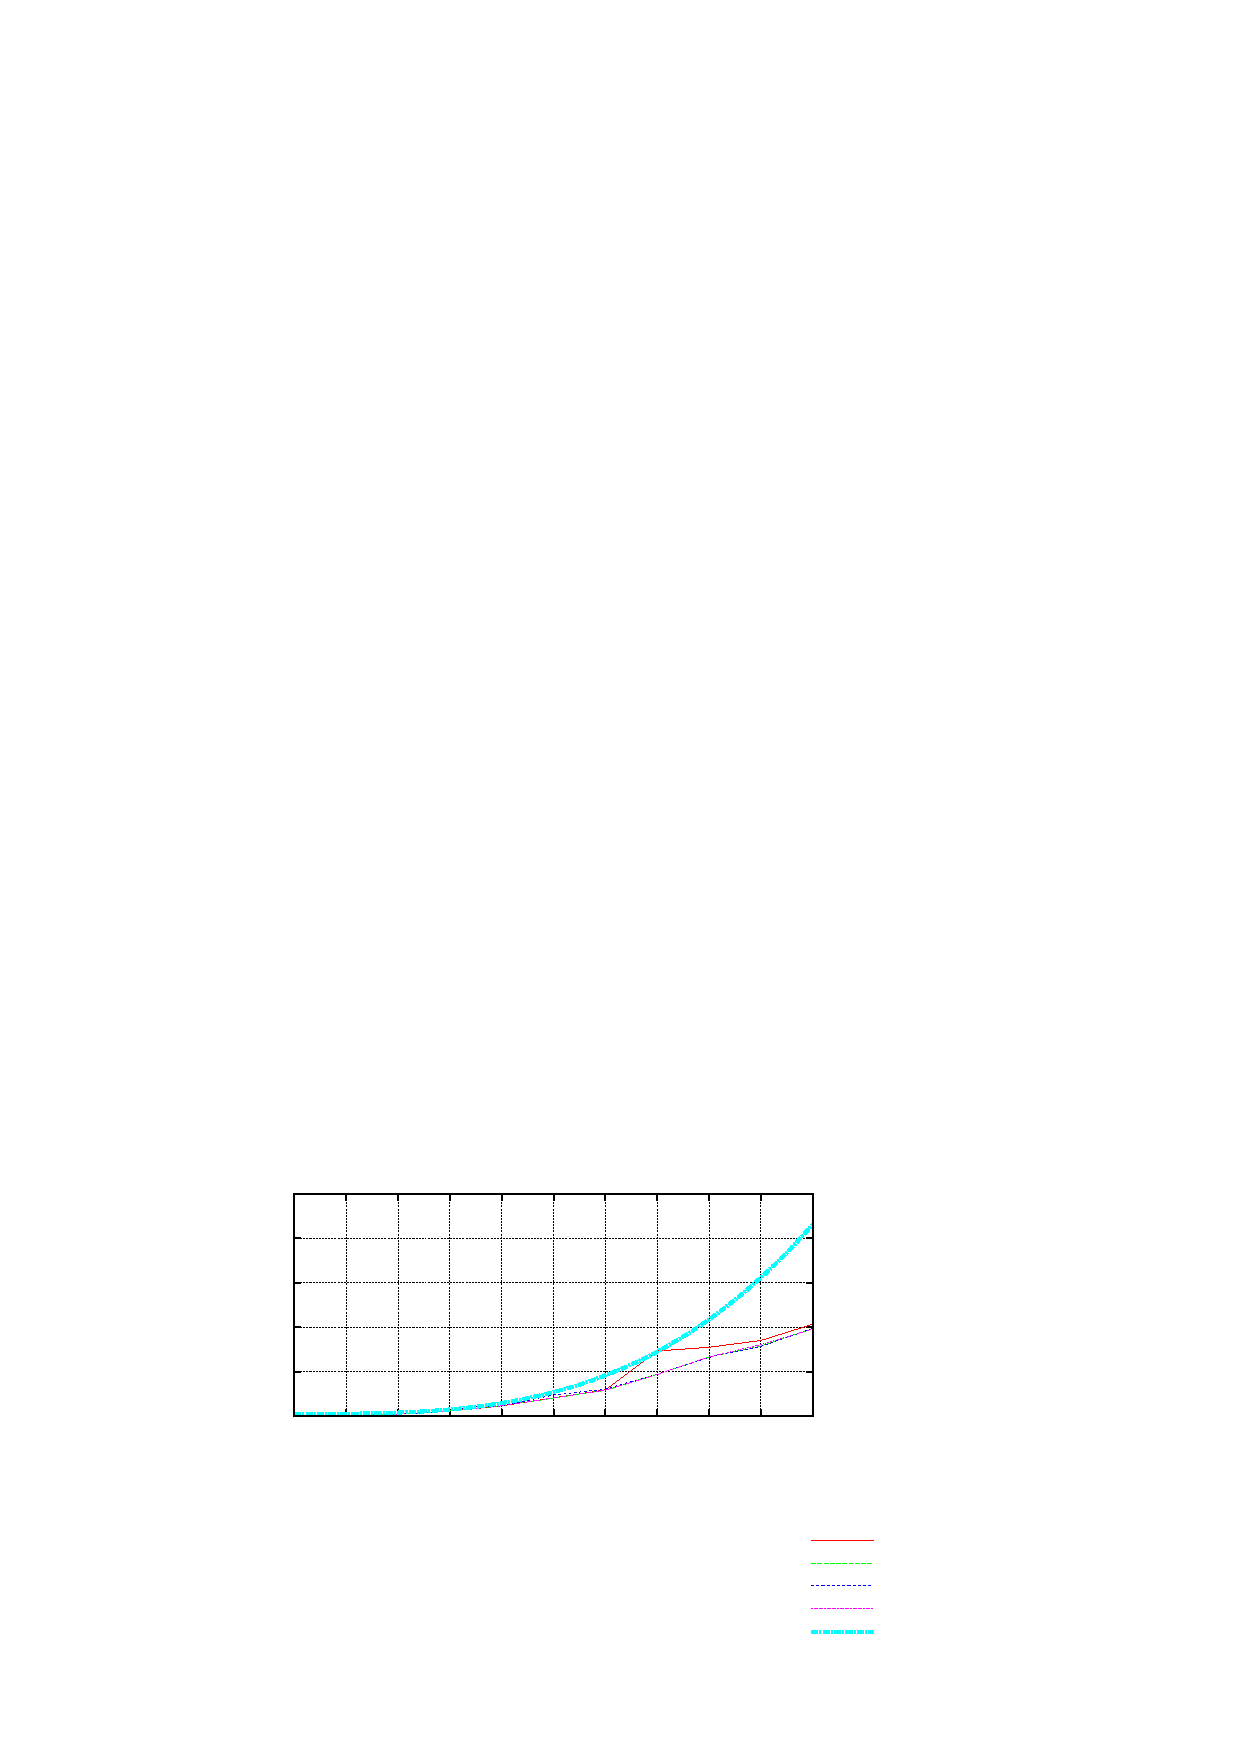
\includegraphics{ej3_nodos_nlogn_complete_bipartite_sin_aspiracion}}%
    \gplfronttext
  \end{picture}%
\endgroup
}
    \caption{Complejidad temporal para grafos Bipartito Completo (Variante Max\_Iter=nlog(n),sin aspiraci\'on)}
\end{figure}

\begin{figure}[H]
    \centering
    \fontsize{8}{10}\selectfont
    \resizebox{0.8\textwidth}{!}{% GNUPLOT: LaTeX picture with Postscript
\begingroup
  \makeatletter
  \providecommand\color[2][]{%
    \GenericError{(gnuplot) \space\space\space\@spaces}{%
      Package color not loaded in conjunction with
      terminal option `colourtext'%
    }{See the gnuplot documentation for explanation.%
    }{Either use 'blacktext' in gnuplot or load the package
      color.sty in LaTeX.}%
    \renewcommand\color[2][]{}%
  }%
  \providecommand\includegraphics[2][]{%
    \GenericError{(gnuplot) \space\space\space\@spaces}{%
      Package graphicx or graphics not loaded%
    }{See the gnuplot documentation for explanation.%
    }{The gnuplot epslatex terminal needs graphicx.sty or graphics.sty.}%
    \renewcommand\includegraphics[2][]{}%
  }%
  \providecommand\rotatebox[2]{#2}%
  \@ifundefined{ifGPcolor}{%
    \newif\ifGPcolor
    \GPcolortrue
  }{}%
  \@ifundefined{ifGPblacktext}{%
    \newif\ifGPblacktext
    \GPblacktexttrue
  }{}%
  % define a \g@addto@macro without @ in the name:
  \let\gplgaddtomacro\g@addto@macro
  % define empty templates for all commands taking text:
  \gdef\gplbacktext{}%
  \gdef\gplfronttext{}%
  \makeatother
  \ifGPblacktext
    % no textcolor at all
    \def\colorrgb#1{}%
    \def\colorgray#1{}%
  \else
    % gray or color?
    \ifGPcolor
      \def\colorrgb#1{\color[rgb]{#1}}%
      \def\colorgray#1{\color[gray]{#1}}%
      \expandafter\def\csname LTw\endcsname{\color{white}}%
      \expandafter\def\csname LTb\endcsname{\color{black}}%
      \expandafter\def\csname LTa\endcsname{\color{black}}%
      \expandafter\def\csname LT0\endcsname{\color[rgb]{1,0,0}}%
      \expandafter\def\csname LT1\endcsname{\color[rgb]{0,1,0}}%
      \expandafter\def\csname LT2\endcsname{\color[rgb]{0,0,1}}%
      \expandafter\def\csname LT3\endcsname{\color[rgb]{1,0,1}}%
      \expandafter\def\csname LT4\endcsname{\color[rgb]{0,1,1}}%
      \expandafter\def\csname LT5\endcsname{\color[rgb]{1,1,0}}%
      \expandafter\def\csname LT6\endcsname{\color[rgb]{0,0,0}}%
      \expandafter\def\csname LT7\endcsname{\color[rgb]{1,0.3,0}}%
      \expandafter\def\csname LT8\endcsname{\color[rgb]{0.5,0.5,0.5}}%
    \else
      % gray
      \def\colorrgb#1{\color{black}}%
      \def\colorgray#1{\color[gray]{#1}}%
      \expandafter\def\csname LTw\endcsname{\color{white}}%
      \expandafter\def\csname LTb\endcsname{\color{black}}%
      \expandafter\def\csname LTa\endcsname{\color{black}}%
      \expandafter\def\csname LT0\endcsname{\color{black}}%
      \expandafter\def\csname LT1\endcsname{\color{black}}%
      \expandafter\def\csname LT2\endcsname{\color{black}}%
      \expandafter\def\csname LT3\endcsname{\color{black}}%
      \expandafter\def\csname LT4\endcsname{\color{black}}%
      \expandafter\def\csname LT5\endcsname{\color{black}}%
      \expandafter\def\csname LT6\endcsname{\color{black}}%
      \expandafter\def\csname LT7\endcsname{\color{black}}%
      \expandafter\def\csname LT8\endcsname{\color{black}}%
    \fi
  \fi
  \setlength{\unitlength}{0.0500bp}%
  \begin{picture}(7200.00,5040.00)%
    \gplgaddtomacro\gplbacktext{%
      \csname LTb\endcsname%
      \put(1694,2244){\makebox(0,0)[r]{\strut{} 0}}%
      \csname LTb\endcsname%
      \put(1694,2511){\makebox(0,0)[r]{\strut{} 200000}}%
      \csname LTb\endcsname%
      \put(1694,2778){\makebox(0,0)[r]{\strut{} 400000}}%
      \csname LTb\endcsname%
      \put(1694,3045){\makebox(0,0)[r]{\strut{} 600000}}%
      \csname LTb\endcsname%
      \put(1694,3312){\makebox(0,0)[r]{\strut{} 800000}}%
      \csname LTb\endcsname%
      \put(1694,3578){\makebox(0,0)[r]{\strut{} 1e+06}}%
      \csname LTb\endcsname%
      \put(1694,3845){\makebox(0,0)[r]{\strut{} 1.2e+06}}%
      \csname LTb\endcsname%
      \put(1694,4112){\makebox(0,0)[r]{\strut{} 1.4e+06}}%
      \csname LTb\endcsname%
      \put(1694,4379){\makebox(0,0)[r]{\strut{} 1.6e+06}}%
      \csname LTb\endcsname%
      \put(1826,2024){\makebox(0,0){\strut{} 0}}%
      \csname LTb\endcsname%
      \put(2324,2024){\makebox(0,0){\strut{} 500}}%
      \csname LTb\endcsname%
      \put(2821,2024){\makebox(0,0){\strut{} 1000}}%
      \csname LTb\endcsname%
      \put(3319,2024){\makebox(0,0){\strut{} 1500}}%
      \csname LTb\endcsname%
      \put(3817,2024){\makebox(0,0){\strut{} 2000}}%
      \csname LTb\endcsname%
      \put(4315,2024){\makebox(0,0){\strut{} 2500}}%
      \csname LTb\endcsname%
      \put(4812,2024){\makebox(0,0){\strut{} 3000}}%
      \csname LTb\endcsname%
      \put(5310,2024){\makebox(0,0){\strut{} 3500}}%
      \csname LTb\endcsname%
      \put(5808,2024){\makebox(0,0){\strut{} 4000}}%
      \csname LTb\endcsname%
      \put(6305,2024){\makebox(0,0){\strut{} 4500}}%
      \csname LTb\endcsname%
      \put(6803,2024){\makebox(0,0){\strut{} 5000}}%
      \put(176,3311){\rotatebox{-270}{\makebox(0,0){\strut{}Tiempo (microsegundos)}}}%
      \put(396,3311){\rotatebox{-270}{\makebox(0,0){\strut{}(Escala Lineal)}}}%
      \put(4314,1694){\makebox(0,0){\strut{}Cantidad de Nodos}}%
      \put(4314,1474){\makebox(0,0){\strut{}(Escala Lineal)}}%
      \put(4314,4709){\makebox(0,0){\strut{}Tiempo de ejecucion conforme aumenta la cantidad de nodos}}%
    }%
    \gplgaddtomacro\gplfronttext{%
      \csname LTb\endcsname%
      \put(6263,1053){\makebox(0,0)[r]{\strut{}Iter=n,Sin Mejorar=n,Tiempo Tabu=n}}%
      \csname LTb\endcsname%
      \put(6263,833){\makebox(0,0)[r]{\strut{}Iter=n,Sin Mejorar=n,Tiempo Tabu=n2}}%
      \csname LTb\endcsname%
      \put(6263,613){\makebox(0,0)[r]{\strut{}Iter=n,Sin Mejorar=n2,Tiempo Tabu=n}}%
      \csname LTb\endcsname%
      \put(6263,393){\makebox(0,0)[r]{\strut{}Iter=n,Sin Mejorar=n2,Tiempo Tabu=n2}}%
      \csname LTb\endcsname%
      \put(6263,173){\makebox(0,0)[r]{\strut{}Cota teórica superior $\mathcal O(n^3)$}}%
    }%
    \gplbacktext
    \put(0,0){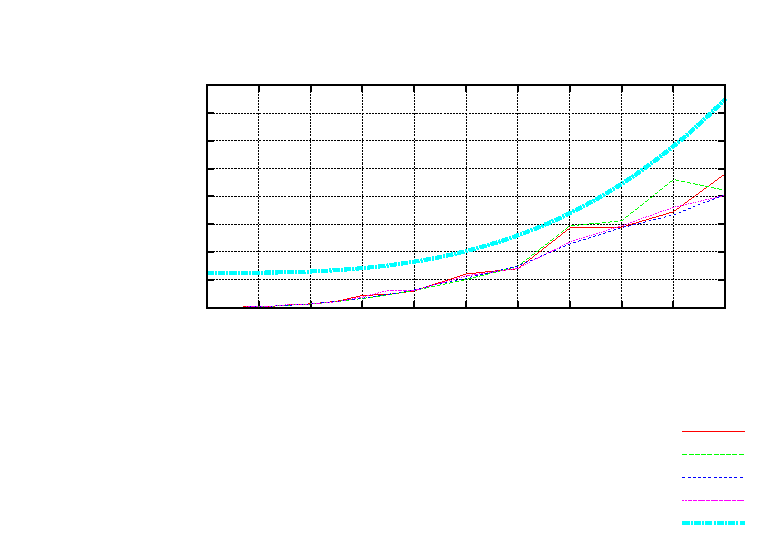
\includegraphics{ej3_nodos_n_complete_bipartite_sin_aspiracion}}%
    \gplfronttext
  \end{picture}%
\endgroup
}
    \caption{Complejidad temporal para grafos Bipartito Completo (Variante Max\_Iter=n),sin aspiraci\'on)}
\end{figure}

\begin{figure}[H]
    \centering
    \fontsize{8}{10}\selectfont
    \resizebox{0.8\textwidth}{!}{% GNUPLOT: LaTeX picture with Postscript
\begingroup
  \makeatletter
  \providecommand\color[2][]{%
    \GenericError{(gnuplot) \space\space\space\@spaces}{%
      Package color not loaded in conjunction with
      terminal option `colourtext'%
    }{See the gnuplot documentation for explanation.%
    }{Either use 'blacktext' in gnuplot or load the package
      color.sty in LaTeX.}%
    \renewcommand\color[2][]{}%
  }%
  \providecommand\includegraphics[2][]{%
    \GenericError{(gnuplot) \space\space\space\@spaces}{%
      Package graphicx or graphics not loaded%
    }{See the gnuplot documentation for explanation.%
    }{The gnuplot epslatex terminal needs graphicx.sty or graphics.sty.}%
    \renewcommand\includegraphics[2][]{}%
  }%
  \providecommand\rotatebox[2]{#2}%
  \@ifundefined{ifGPcolor}{%
    \newif\ifGPcolor
    \GPcolortrue
  }{}%
  \@ifundefined{ifGPblacktext}{%
    \newif\ifGPblacktext
    \GPblacktexttrue
  }{}%
  % define a \g@addto@macro without @ in the name:
  \let\gplgaddtomacro\g@addto@macro
  % define empty templates for all commands taking text:
  \gdef\gplbacktext{}%
  \gdef\gplfronttext{}%
  \makeatother
  \ifGPblacktext
    % no textcolor at all
    \def\colorrgb#1{}%
    \def\colorgray#1{}%
  \else
    % gray or color?
    \ifGPcolor
      \def\colorrgb#1{\color[rgb]{#1}}%
      \def\colorgray#1{\color[gray]{#1}}%
      \expandafter\def\csname LTw\endcsname{\color{white}}%
      \expandafter\def\csname LTb\endcsname{\color{black}}%
      \expandafter\def\csname LTa\endcsname{\color{black}}%
      \expandafter\def\csname LT0\endcsname{\color[rgb]{1,0,0}}%
      \expandafter\def\csname LT1\endcsname{\color[rgb]{0,1,0}}%
      \expandafter\def\csname LT2\endcsname{\color[rgb]{0,0,1}}%
      \expandafter\def\csname LT3\endcsname{\color[rgb]{1,0,1}}%
      \expandafter\def\csname LT4\endcsname{\color[rgb]{0,1,1}}%
      \expandafter\def\csname LT5\endcsname{\color[rgb]{1,1,0}}%
      \expandafter\def\csname LT6\endcsname{\color[rgb]{0,0,0}}%
      \expandafter\def\csname LT7\endcsname{\color[rgb]{1,0.3,0}}%
      \expandafter\def\csname LT8\endcsname{\color[rgb]{0.5,0.5,0.5}}%
    \else
      % gray
      \def\colorrgb#1{\color{black}}%
      \def\colorgray#1{\color[gray]{#1}}%
      \expandafter\def\csname LTw\endcsname{\color{white}}%
      \expandafter\def\csname LTb\endcsname{\color{black}}%
      \expandafter\def\csname LTa\endcsname{\color{black}}%
      \expandafter\def\csname LT0\endcsname{\color{black}}%
      \expandafter\def\csname LT1\endcsname{\color{black}}%
      \expandafter\def\csname LT2\endcsname{\color{black}}%
      \expandafter\def\csname LT3\endcsname{\color{black}}%
      \expandafter\def\csname LT4\endcsname{\color{black}}%
      \expandafter\def\csname LT5\endcsname{\color{black}}%
      \expandafter\def\csname LT6\endcsname{\color{black}}%
      \expandafter\def\csname LT7\endcsname{\color{black}}%
      \expandafter\def\csname LT8\endcsname{\color{black}}%
    \fi
  \fi
  \setlength{\unitlength}{0.0500bp}%
  \begin{picture}(7200.00,5040.00)%
    \gplgaddtomacro\gplbacktext{%
      \csname LTb\endcsname%
      \put(1298,2904){\makebox(0,0)[r]{\strut{} 0}}%
      \csname LTb\endcsname%
      \put(1298,3052){\makebox(0,0)[r]{\strut{} 500}}%
      \csname LTb\endcsname%
      \put(1298,3199){\makebox(0,0)[r]{\strut{} 1000}}%
      \csname LTb\endcsname%
      \put(1298,3347){\makebox(0,0)[r]{\strut{} 1500}}%
      \csname LTb\endcsname%
      \put(1298,3494){\makebox(0,0)[r]{\strut{} 2000}}%
      \csname LTb\endcsname%
      \put(1298,3642){\makebox(0,0)[r]{\strut{} 2500}}%
      \csname LTb\endcsname%
      \put(1298,3789){\makebox(0,0)[r]{\strut{} 3000}}%
      \csname LTb\endcsname%
      \put(1298,3937){\makebox(0,0)[r]{\strut{} 3500}}%
      \csname LTb\endcsname%
      \put(1298,4084){\makebox(0,0)[r]{\strut{} 4000}}%
      \csname LTb\endcsname%
      \put(1298,4232){\makebox(0,0)[r]{\strut{} 4500}}%
      \csname LTb\endcsname%
      \put(1298,4379){\makebox(0,0)[r]{\strut{} 5000}}%
      \csname LTb\endcsname%
      \put(1430,2684){\makebox(0,0){\strut{} 0}}%
      \csname LTb\endcsname%
      \put(1967,2684){\makebox(0,0){\strut{} 500}}%
      \csname LTb\endcsname%
      \put(2505,2684){\makebox(0,0){\strut{} 1000}}%
      \csname LTb\endcsname%
      \put(3042,2684){\makebox(0,0){\strut{} 1500}}%
      \csname LTb\endcsname%
      \put(3579,2684){\makebox(0,0){\strut{} 2000}}%
      \csname LTb\endcsname%
      \put(4117,2684){\makebox(0,0){\strut{} 2500}}%
      \csname LTb\endcsname%
      \put(4654,2684){\makebox(0,0){\strut{} 3000}}%
      \csname LTb\endcsname%
      \put(5191,2684){\makebox(0,0){\strut{} 3500}}%
      \csname LTb\endcsname%
      \put(5728,2684){\makebox(0,0){\strut{} 4000}}%
      \csname LTb\endcsname%
      \put(6266,2684){\makebox(0,0){\strut{} 4500}}%
      \csname LTb\endcsname%
      \put(6803,2684){\makebox(0,0){\strut{} 5000}}%
      \put(176,3641){\rotatebox{-270}{\makebox(0,0){\strut{}Frontera}}}%
      \put(396,3641){\rotatebox{-270}{\makebox(0,0){\strut{}(Escala Lineal)}}}%
      \put(4116,2354){\makebox(0,0){\strut{}Cantidad de Nodos}}%
      \put(4116,2134){\makebox(0,0){\strut{}(Escala Lineal)}}%
      \put(4116,4709){\makebox(0,0){\strut{}Frontera obtenida segun cantidad de nodos}}%
    }%
    \gplgaddtomacro\gplfronttext{%
      \csname LTb\endcsname%
      \put(6461,1713){\makebox(0,0)[r]{\strut{}Iter=nlog(n),Sin Mejorar=n,Tiempo Tabu=n}}%
      \csname LTb\endcsname%
      \put(6461,1493){\makebox(0,0)[r]{\strut{}Iter=nlog(n),Sin Mejorar=n,Tiempo Tabu=n2}}%
      \csname LTb\endcsname%
      \put(6461,1273){\makebox(0,0)[r]{\strut{}Iter=nlog(n),Sin Mejorar=n2,Tiempo Tabu=n}}%
      \csname LTb\endcsname%
      \put(6461,1053){\makebox(0,0)[r]{\strut{}Iter=nlog(n),Sin Mejorar=n2,Tiempo Tabu=n2}}%
      \csname LTb\endcsname%
      \put(6461,833){\makebox(0,0)[r]{\strut{}Iter=n,Sin Mejorar=n,Tiempo Tabu=n}}%
      \csname LTb\endcsname%
      \put(6461,613){\makebox(0,0)[r]{\strut{}Iter=n,Sin Mejorar=n,Tiempo Tabu=n2}}%
      \csname LTb\endcsname%
      \put(6461,393){\makebox(0,0)[r]{\strut{}Iter=n,Sin Mejorar=n2,Tiempo Tabu=n}}%
      \csname LTb\endcsname%
      \put(6461,173){\makebox(0,0)[r]{\strut{}Iter=n,Sin Mejorar=n2,Tiempo Tabu=n2}}%
    }%
    \gplbacktext
    \put(0,0){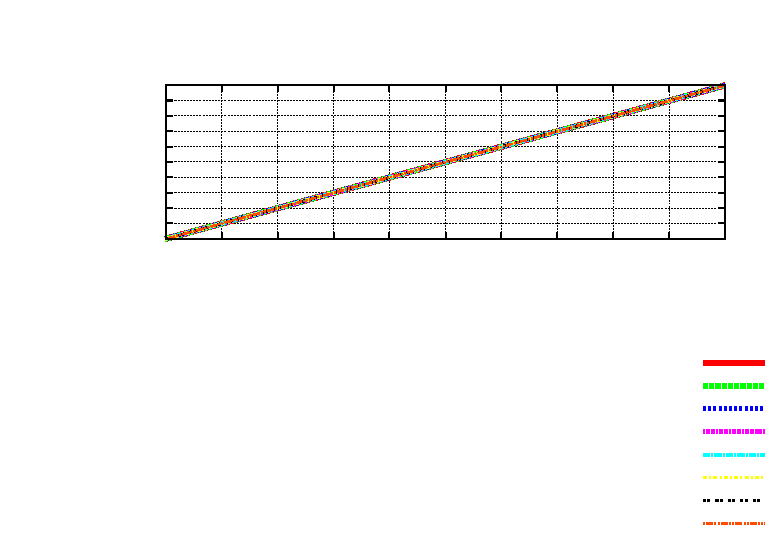
\includegraphics{ej3_frontera_complete_bipartite_sin_aspiracion}}%
    \gplfronttext
  \end{picture}%
\endgroup
}
    \caption{Frontera de grafos Bipartito Completo (sin aspiracion)}
\end{figure}

%Bipartito Completo sin aspiracion golosa
\begin{figure}[H]
    \centering
    \fontsize{8}{10}\selectfont
    \resizebox{0.8\textwidth}{!}{% GNUPLOT: LaTeX picture with Postscript
\begingroup
  \makeatletter
  \providecommand\color[2][]{%
    \GenericError{(gnuplot) \space\space\space\@spaces}{%
      Package color not loaded in conjunction with
      terminal option `colourtext'%
    }{See the gnuplot documentation for explanation.%
    }{Either use 'blacktext' in gnuplot or load the package
      color.sty in LaTeX.}%
    \renewcommand\color[2][]{}%
  }%
  \providecommand\includegraphics[2][]{%
    \GenericError{(gnuplot) \space\space\space\@spaces}{%
      Package graphicx or graphics not loaded%
    }{See the gnuplot documentation for explanation.%
    }{The gnuplot epslatex terminal needs graphicx.sty or graphics.sty.}%
    \renewcommand\includegraphics[2][]{}%
  }%
  \providecommand\rotatebox[2]{#2}%
  \@ifundefined{ifGPcolor}{%
    \newif\ifGPcolor
    \GPcolortrue
  }{}%
  \@ifundefined{ifGPblacktext}{%
    \newif\ifGPblacktext
    \GPblacktexttrue
  }{}%
  % define a \g@addto@macro without @ in the name:
  \let\gplgaddtomacro\g@addto@macro
  % define empty templates for all commands taking text:
  \gdef\gplbacktext{}%
  \gdef\gplfronttext{}%
  \makeatother
  \ifGPblacktext
    % no textcolor at all
    \def\colorrgb#1{}%
    \def\colorgray#1{}%
  \else
    % gray or color?
    \ifGPcolor
      \def\colorrgb#1{\color[rgb]{#1}}%
      \def\colorgray#1{\color[gray]{#1}}%
      \expandafter\def\csname LTw\endcsname{\color{white}}%
      \expandafter\def\csname LTb\endcsname{\color{black}}%
      \expandafter\def\csname LTa\endcsname{\color{black}}%
      \expandafter\def\csname LT0\endcsname{\color[rgb]{1,0,0}}%
      \expandafter\def\csname LT1\endcsname{\color[rgb]{0,1,0}}%
      \expandafter\def\csname LT2\endcsname{\color[rgb]{0,0,1}}%
      \expandafter\def\csname LT3\endcsname{\color[rgb]{1,0,1}}%
      \expandafter\def\csname LT4\endcsname{\color[rgb]{0,1,1}}%
      \expandafter\def\csname LT5\endcsname{\color[rgb]{1,1,0}}%
      \expandafter\def\csname LT6\endcsname{\color[rgb]{0,0,0}}%
      \expandafter\def\csname LT7\endcsname{\color[rgb]{1,0.3,0}}%
      \expandafter\def\csname LT8\endcsname{\color[rgb]{0.5,0.5,0.5}}%
    \else
      % gray
      \def\colorrgb#1{\color{black}}%
      \def\colorgray#1{\color[gray]{#1}}%
      \expandafter\def\csname LTw\endcsname{\color{white}}%
      \expandafter\def\csname LTb\endcsname{\color{black}}%
      \expandafter\def\csname LTa\endcsname{\color{black}}%
      \expandafter\def\csname LT0\endcsname{\color{black}}%
      \expandafter\def\csname LT1\endcsname{\color{black}}%
      \expandafter\def\csname LT2\endcsname{\color{black}}%
      \expandafter\def\csname LT3\endcsname{\color{black}}%
      \expandafter\def\csname LT4\endcsname{\color{black}}%
      \expandafter\def\csname LT5\endcsname{\color{black}}%
      \expandafter\def\csname LT6\endcsname{\color{black}}%
      \expandafter\def\csname LT7\endcsname{\color{black}}%
      \expandafter\def\csname LT8\endcsname{\color{black}}%
    \fi
  \fi
  \setlength{\unitlength}{0.0500bp}%
  \begin{picture}(7200.00,5040.00)%
    \gplgaddtomacro\gplbacktext{%
      \csname LTb\endcsname%
      \put(1694,2244){\makebox(0,0)[r]{\strut{} 0}}%
      \csname LTb\endcsname%
      \put(1694,2671){\makebox(0,0)[r]{\strut{} 5e+06}}%
      \csname LTb\endcsname%
      \put(1694,3098){\makebox(0,0)[r]{\strut{} 1e+07}}%
      \csname LTb\endcsname%
      \put(1694,3525){\makebox(0,0)[r]{\strut{} 1.5e+07}}%
      \csname LTb\endcsname%
      \put(1694,3952){\makebox(0,0)[r]{\strut{} 2e+07}}%
      \csname LTb\endcsname%
      \put(1694,4379){\makebox(0,0)[r]{\strut{} 2.5e+07}}%
      \csname LTb\endcsname%
      \put(1826,2024){\makebox(0,0){\strut{} 0}}%
      \csname LTb\endcsname%
      \put(2324,2024){\makebox(0,0){\strut{} 500}}%
      \csname LTb\endcsname%
      \put(2821,2024){\makebox(0,0){\strut{} 1000}}%
      \csname LTb\endcsname%
      \put(3319,2024){\makebox(0,0){\strut{} 1500}}%
      \csname LTb\endcsname%
      \put(3817,2024){\makebox(0,0){\strut{} 2000}}%
      \csname LTb\endcsname%
      \put(4315,2024){\makebox(0,0){\strut{} 2500}}%
      \csname LTb\endcsname%
      \put(4812,2024){\makebox(0,0){\strut{} 3000}}%
      \csname LTb\endcsname%
      \put(5310,2024){\makebox(0,0){\strut{} 3500}}%
      \csname LTb\endcsname%
      \put(5808,2024){\makebox(0,0){\strut{} 4000}}%
      \csname LTb\endcsname%
      \put(6305,2024){\makebox(0,0){\strut{} 4500}}%
      \csname LTb\endcsname%
      \put(6803,2024){\makebox(0,0){\strut{} 5000}}%
      \put(176,3311){\rotatebox{-270}{\makebox(0,0){\strut{}Tiempo (microsegundos)}}}%
      \put(396,3311){\rotatebox{-270}{\makebox(0,0){\strut{}(Escala Lineal)}}}%
      \put(4314,1694){\makebox(0,0){\strut{}Cantidad de Nodos}}%
      \put(4314,1474){\makebox(0,0){\strut{}(Escala Lineal)}}%
      \put(4314,4709){\makebox(0,0){\strut{}Tiempo de ejecucion conforme aumenta la cantidad de nodos}}%
    }%
    \gplgaddtomacro\gplfronttext{%
      \csname LTb\endcsname%
      \put(6659,1053){\makebox(0,0)[r]{\strut{}Iter=nlog(n),Sin Mejorar=n,Tiempo Tabu=n}}%
      \csname LTb\endcsname%
      \put(6659,833){\makebox(0,0)[r]{\strut{}Iter=nlog(n),Sin Mejorar=n,Tiempo Tabu=n2}}%
      \csname LTb\endcsname%
      \put(6659,613){\makebox(0,0)[r]{\strut{}Iter=nlog(n),Sin Mejorar=n2,Tiempo Tabu=n}}%
      \csname LTb\endcsname%
      \put(6659,393){\makebox(0,0)[r]{\strut{}Iter=nlog(n),Sin Mejorar=n2,Tiempo Tabu=n2}}%
      \csname LTb\endcsname%
      \put(6659,173){\makebox(0,0)[r]{\strut{}Cota teórica superior $\mathcal O(n^3 \cdot log(n))$}}%
    }%
    \gplbacktext
    \put(0,0){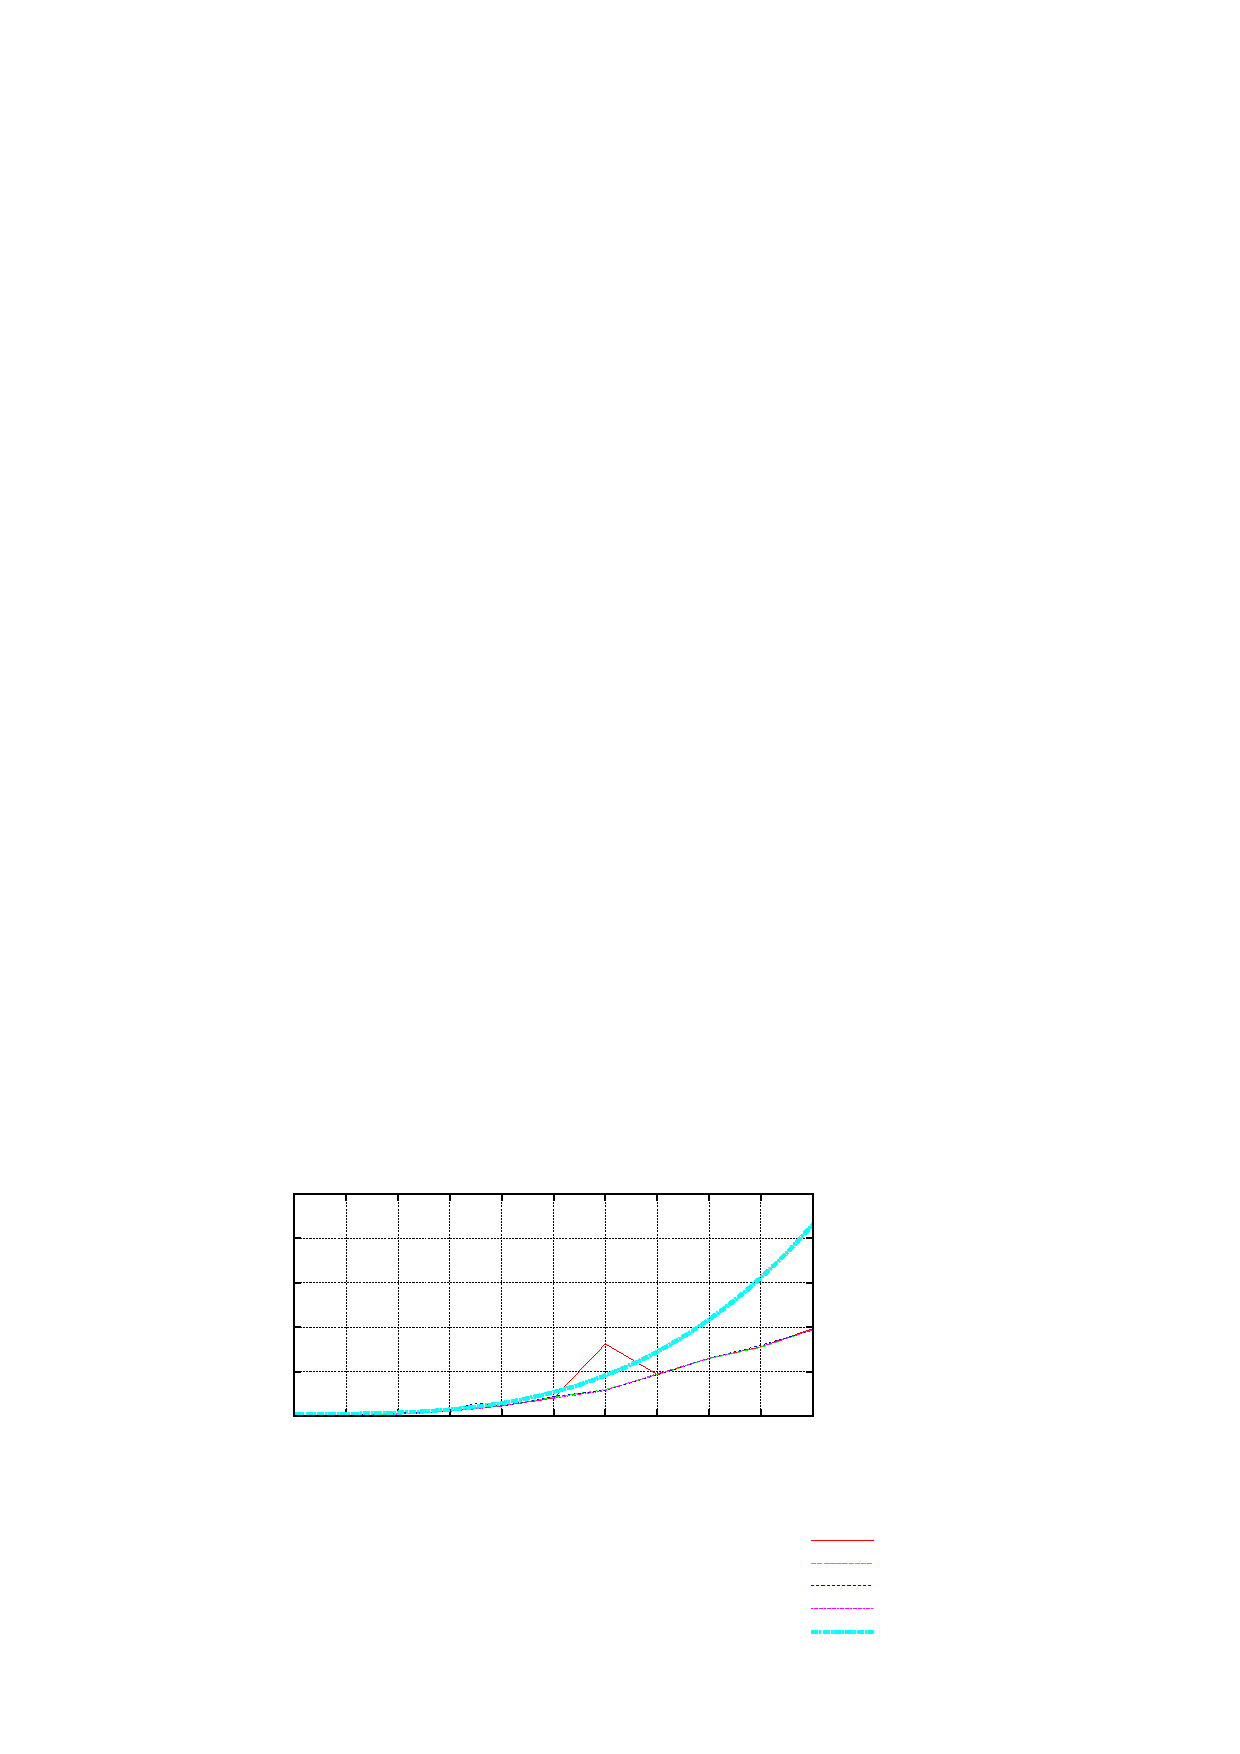
\includegraphics{ej3_nodos_nlogn_complete_bipartite_sin_aspiracion_golosa}}%
    \gplfronttext
  \end{picture}%
\endgroup
}
    \caption{Complejidad temporal para grafos Bipartito Completo (Variante Max\_Iter=nlog(n),sin aspiraci\'on,golosa)}
\end{figure}

\begin{figure}[H]
    \centering
    \fontsize{8}{10}\selectfont
    \resizebox{0.8\textwidth}{!}{% GNUPLOT: LaTeX picture with Postscript
\begingroup
  \makeatletter
  \providecommand\color[2][]{%
    \GenericError{(gnuplot) \space\space\space\@spaces}{%
      Package color not loaded in conjunction with
      terminal option `colourtext'%
    }{See the gnuplot documentation for explanation.%
    }{Either use 'blacktext' in gnuplot or load the package
      color.sty in LaTeX.}%
    \renewcommand\color[2][]{}%
  }%
  \providecommand\includegraphics[2][]{%
    \GenericError{(gnuplot) \space\space\space\@spaces}{%
      Package graphicx or graphics not loaded%
    }{See the gnuplot documentation for explanation.%
    }{The gnuplot epslatex terminal needs graphicx.sty or graphics.sty.}%
    \renewcommand\includegraphics[2][]{}%
  }%
  \providecommand\rotatebox[2]{#2}%
  \@ifundefined{ifGPcolor}{%
    \newif\ifGPcolor
    \GPcolortrue
  }{}%
  \@ifundefined{ifGPblacktext}{%
    \newif\ifGPblacktext
    \GPblacktexttrue
  }{}%
  % define a \g@addto@macro without @ in the name:
  \let\gplgaddtomacro\g@addto@macro
  % define empty templates for all commands taking text:
  \gdef\gplbacktext{}%
  \gdef\gplfronttext{}%
  \makeatother
  \ifGPblacktext
    % no textcolor at all
    \def\colorrgb#1{}%
    \def\colorgray#1{}%
  \else
    % gray or color?
    \ifGPcolor
      \def\colorrgb#1{\color[rgb]{#1}}%
      \def\colorgray#1{\color[gray]{#1}}%
      \expandafter\def\csname LTw\endcsname{\color{white}}%
      \expandafter\def\csname LTb\endcsname{\color{black}}%
      \expandafter\def\csname LTa\endcsname{\color{black}}%
      \expandafter\def\csname LT0\endcsname{\color[rgb]{1,0,0}}%
      \expandafter\def\csname LT1\endcsname{\color[rgb]{0,1,0}}%
      \expandafter\def\csname LT2\endcsname{\color[rgb]{0,0,1}}%
      \expandafter\def\csname LT3\endcsname{\color[rgb]{1,0,1}}%
      \expandafter\def\csname LT4\endcsname{\color[rgb]{0,1,1}}%
      \expandafter\def\csname LT5\endcsname{\color[rgb]{1,1,0}}%
      \expandafter\def\csname LT6\endcsname{\color[rgb]{0,0,0}}%
      \expandafter\def\csname LT7\endcsname{\color[rgb]{1,0.3,0}}%
      \expandafter\def\csname LT8\endcsname{\color[rgb]{0.5,0.5,0.5}}%
    \else
      % gray
      \def\colorrgb#1{\color{black}}%
      \def\colorgray#1{\color[gray]{#1}}%
      \expandafter\def\csname LTw\endcsname{\color{white}}%
      \expandafter\def\csname LTb\endcsname{\color{black}}%
      \expandafter\def\csname LTa\endcsname{\color{black}}%
      \expandafter\def\csname LT0\endcsname{\color{black}}%
      \expandafter\def\csname LT1\endcsname{\color{black}}%
      \expandafter\def\csname LT2\endcsname{\color{black}}%
      \expandafter\def\csname LT3\endcsname{\color{black}}%
      \expandafter\def\csname LT4\endcsname{\color{black}}%
      \expandafter\def\csname LT5\endcsname{\color{black}}%
      \expandafter\def\csname LT6\endcsname{\color{black}}%
      \expandafter\def\csname LT7\endcsname{\color{black}}%
      \expandafter\def\csname LT8\endcsname{\color{black}}%
    \fi
  \fi
  \setlength{\unitlength}{0.0500bp}%
  \begin{picture}(7200.00,5040.00)%
    \gplgaddtomacro\gplbacktext{%
      \csname LTb\endcsname%
      \put(1694,2244){\makebox(0,0)[r]{\strut{} 0}}%
      \csname LTb\endcsname%
      \put(1694,2511){\makebox(0,0)[r]{\strut{} 200000}}%
      \csname LTb\endcsname%
      \put(1694,2778){\makebox(0,0)[r]{\strut{} 400000}}%
      \csname LTb\endcsname%
      \put(1694,3045){\makebox(0,0)[r]{\strut{} 600000}}%
      \csname LTb\endcsname%
      \put(1694,3312){\makebox(0,0)[r]{\strut{} 800000}}%
      \csname LTb\endcsname%
      \put(1694,3578){\makebox(0,0)[r]{\strut{} 1e+06}}%
      \csname LTb\endcsname%
      \put(1694,3845){\makebox(0,0)[r]{\strut{} 1.2e+06}}%
      \csname LTb\endcsname%
      \put(1694,4112){\makebox(0,0)[r]{\strut{} 1.4e+06}}%
      \csname LTb\endcsname%
      \put(1694,4379){\makebox(0,0)[r]{\strut{} 1.6e+06}}%
      \csname LTb\endcsname%
      \put(1826,2024){\makebox(0,0){\strut{} 0}}%
      \csname LTb\endcsname%
      \put(2324,2024){\makebox(0,0){\strut{} 500}}%
      \csname LTb\endcsname%
      \put(2821,2024){\makebox(0,0){\strut{} 1000}}%
      \csname LTb\endcsname%
      \put(3319,2024){\makebox(0,0){\strut{} 1500}}%
      \csname LTb\endcsname%
      \put(3817,2024){\makebox(0,0){\strut{} 2000}}%
      \csname LTb\endcsname%
      \put(4315,2024){\makebox(0,0){\strut{} 2500}}%
      \csname LTb\endcsname%
      \put(4812,2024){\makebox(0,0){\strut{} 3000}}%
      \csname LTb\endcsname%
      \put(5310,2024){\makebox(0,0){\strut{} 3500}}%
      \csname LTb\endcsname%
      \put(5808,2024){\makebox(0,0){\strut{} 4000}}%
      \csname LTb\endcsname%
      \put(6305,2024){\makebox(0,0){\strut{} 4500}}%
      \csname LTb\endcsname%
      \put(6803,2024){\makebox(0,0){\strut{} 5000}}%
      \put(176,3311){\rotatebox{-270}{\makebox(0,0){\strut{}Tiempo (microsegundos)}}}%
      \put(396,3311){\rotatebox{-270}{\makebox(0,0){\strut{}(Escala Lineal)}}}%
      \put(4314,1694){\makebox(0,0){\strut{}Cantidad de Nodos}}%
      \put(4314,1474){\makebox(0,0){\strut{}(Escala Lineal)}}%
      \put(4314,4709){\makebox(0,0){\strut{}Tiempo de ejecucion conforme aumenta la cantidad de nodos}}%
    }%
    \gplgaddtomacro\gplfronttext{%
      \csname LTb\endcsname%
      \put(6263,1053){\makebox(0,0)[r]{\strut{}Iter=n,Sin Mejorar=n,Tiempo Tabu=n}}%
      \csname LTb\endcsname%
      \put(6263,833){\makebox(0,0)[r]{\strut{}Iter=n,Sin Mejorar=n,Tiempo Tabu=n2}}%
      \csname LTb\endcsname%
      \put(6263,613){\makebox(0,0)[r]{\strut{}Iter=n,Sin Mejorar=n2,Tiempo Tabu=n}}%
      \csname LTb\endcsname%
      \put(6263,393){\makebox(0,0)[r]{\strut{}Iter=n,Sin Mejorar=n2,Tiempo Tabu=n2}}%
      \csname LTb\endcsname%
      \put(6263,173){\makebox(0,0)[r]{\strut{}Cota teórica superior $\mathcal O(n^3)$}}%
    }%
    \gplbacktext
    \put(0,0){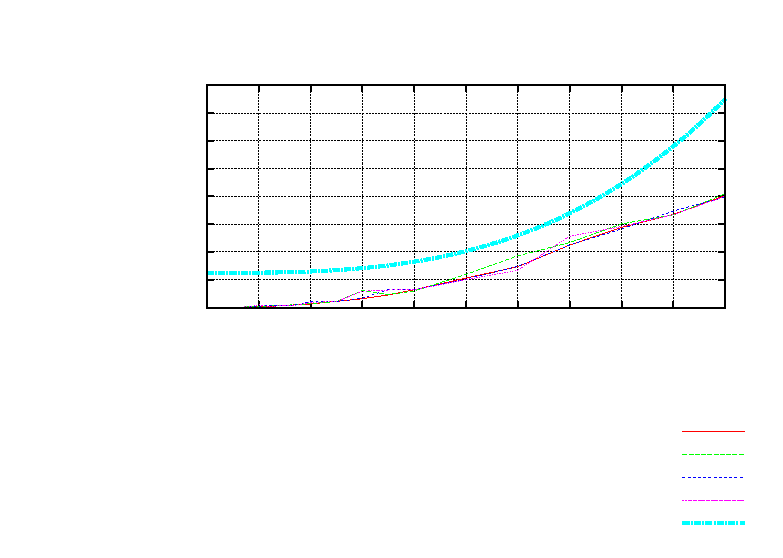
\includegraphics{ej3_nodos_n_complete_bipartite_sin_aspiracion_golosa}}%
    \gplfronttext
  \end{picture}%
\endgroup
}
    \caption{Complejidad temporal para grafos Bipartito Completo (Variante Max\_Iter=n),sin aspiraci\'on,golosa)}
\end{figure}

\begin{figure}[H]
    \centering
    \fontsize{8}{10}\selectfont
    \resizebox{0.8\textwidth}{!}{% GNUPLOT: LaTeX picture with Postscript
\begingroup
  \makeatletter
  \providecommand\color[2][]{%
    \GenericError{(gnuplot) \space\space\space\@spaces}{%
      Package color not loaded in conjunction with
      terminal option `colourtext'%
    }{See the gnuplot documentation for explanation.%
    }{Either use 'blacktext' in gnuplot or load the package
      color.sty in LaTeX.}%
    \renewcommand\color[2][]{}%
  }%
  \providecommand\includegraphics[2][]{%
    \GenericError{(gnuplot) \space\space\space\@spaces}{%
      Package graphicx or graphics not loaded%
    }{See the gnuplot documentation for explanation.%
    }{The gnuplot epslatex terminal needs graphicx.sty or graphics.sty.}%
    \renewcommand\includegraphics[2][]{}%
  }%
  \providecommand\rotatebox[2]{#2}%
  \@ifundefined{ifGPcolor}{%
    \newif\ifGPcolor
    \GPcolortrue
  }{}%
  \@ifundefined{ifGPblacktext}{%
    \newif\ifGPblacktext
    \GPblacktexttrue
  }{}%
  % define a \g@addto@macro without @ in the name:
  \let\gplgaddtomacro\g@addto@macro
  % define empty templates for all commands taking text:
  \gdef\gplbacktext{}%
  \gdef\gplfronttext{}%
  \makeatother
  \ifGPblacktext
    % no textcolor at all
    \def\colorrgb#1{}%
    \def\colorgray#1{}%
  \else
    % gray or color?
    \ifGPcolor
      \def\colorrgb#1{\color[rgb]{#1}}%
      \def\colorgray#1{\color[gray]{#1}}%
      \expandafter\def\csname LTw\endcsname{\color{white}}%
      \expandafter\def\csname LTb\endcsname{\color{black}}%
      \expandafter\def\csname LTa\endcsname{\color{black}}%
      \expandafter\def\csname LT0\endcsname{\color[rgb]{1,0,0}}%
      \expandafter\def\csname LT1\endcsname{\color[rgb]{0,1,0}}%
      \expandafter\def\csname LT2\endcsname{\color[rgb]{0,0,1}}%
      \expandafter\def\csname LT3\endcsname{\color[rgb]{1,0,1}}%
      \expandafter\def\csname LT4\endcsname{\color[rgb]{0,1,1}}%
      \expandafter\def\csname LT5\endcsname{\color[rgb]{1,1,0}}%
      \expandafter\def\csname LT6\endcsname{\color[rgb]{0,0,0}}%
      \expandafter\def\csname LT7\endcsname{\color[rgb]{1,0.3,0}}%
      \expandafter\def\csname LT8\endcsname{\color[rgb]{0.5,0.5,0.5}}%
    \else
      % gray
      \def\colorrgb#1{\color{black}}%
      \def\colorgray#1{\color[gray]{#1}}%
      \expandafter\def\csname LTw\endcsname{\color{white}}%
      \expandafter\def\csname LTb\endcsname{\color{black}}%
      \expandafter\def\csname LTa\endcsname{\color{black}}%
      \expandafter\def\csname LT0\endcsname{\color{black}}%
      \expandafter\def\csname LT1\endcsname{\color{black}}%
      \expandafter\def\csname LT2\endcsname{\color{black}}%
      \expandafter\def\csname LT3\endcsname{\color{black}}%
      \expandafter\def\csname LT4\endcsname{\color{black}}%
      \expandafter\def\csname LT5\endcsname{\color{black}}%
      \expandafter\def\csname LT6\endcsname{\color{black}}%
      \expandafter\def\csname LT7\endcsname{\color{black}}%
      \expandafter\def\csname LT8\endcsname{\color{black}}%
    \fi
  \fi
  \setlength{\unitlength}{0.0500bp}%
  \begin{picture}(7200.00,5040.00)%
    \gplgaddtomacro\gplbacktext{%
      \csname LTb\endcsname%
      \put(1298,2904){\makebox(0,0)[r]{\strut{} 0}}%
      \csname LTb\endcsname%
      \put(1298,3052){\makebox(0,0)[r]{\strut{} 500}}%
      \csname LTb\endcsname%
      \put(1298,3199){\makebox(0,0)[r]{\strut{} 1000}}%
      \csname LTb\endcsname%
      \put(1298,3347){\makebox(0,0)[r]{\strut{} 1500}}%
      \csname LTb\endcsname%
      \put(1298,3494){\makebox(0,0)[r]{\strut{} 2000}}%
      \csname LTb\endcsname%
      \put(1298,3642){\makebox(0,0)[r]{\strut{} 2500}}%
      \csname LTb\endcsname%
      \put(1298,3789){\makebox(0,0)[r]{\strut{} 3000}}%
      \csname LTb\endcsname%
      \put(1298,3937){\makebox(0,0)[r]{\strut{} 3500}}%
      \csname LTb\endcsname%
      \put(1298,4084){\makebox(0,0)[r]{\strut{} 4000}}%
      \csname LTb\endcsname%
      \put(1298,4232){\makebox(0,0)[r]{\strut{} 4500}}%
      \csname LTb\endcsname%
      \put(1298,4379){\makebox(0,0)[r]{\strut{} 5000}}%
      \csname LTb\endcsname%
      \put(1430,2684){\makebox(0,0){\strut{} 0}}%
      \csname LTb\endcsname%
      \put(1967,2684){\makebox(0,0){\strut{} 500}}%
      \csname LTb\endcsname%
      \put(2505,2684){\makebox(0,0){\strut{} 1000}}%
      \csname LTb\endcsname%
      \put(3042,2684){\makebox(0,0){\strut{} 1500}}%
      \csname LTb\endcsname%
      \put(3579,2684){\makebox(0,0){\strut{} 2000}}%
      \csname LTb\endcsname%
      \put(4117,2684){\makebox(0,0){\strut{} 2500}}%
      \csname LTb\endcsname%
      \put(4654,2684){\makebox(0,0){\strut{} 3000}}%
      \csname LTb\endcsname%
      \put(5191,2684){\makebox(0,0){\strut{} 3500}}%
      \csname LTb\endcsname%
      \put(5728,2684){\makebox(0,0){\strut{} 4000}}%
      \csname LTb\endcsname%
      \put(6266,2684){\makebox(0,0){\strut{} 4500}}%
      \csname LTb\endcsname%
      \put(6803,2684){\makebox(0,0){\strut{} 5000}}%
      \put(176,3641){\rotatebox{-270}{\makebox(0,0){\strut{}Frontera}}}%
      \put(396,3641){\rotatebox{-270}{\makebox(0,0){\strut{}(Escala Lineal)}}}%
      \put(4116,2354){\makebox(0,0){\strut{}Cantidad de Nodos}}%
      \put(4116,2134){\makebox(0,0){\strut{}(Escala Lineal)}}%
      \put(4116,4709){\makebox(0,0){\strut{}Frontera obtenida segun cantidad de nodos}}%
    }%
    \gplgaddtomacro\gplfronttext{%
      \csname LTb\endcsname%
      \put(6461,1713){\makebox(0,0)[r]{\strut{}Iter=nlog(n),Sin Mejorar=n,Tiempo Tabu=n}}%
      \csname LTb\endcsname%
      \put(6461,1493){\makebox(0,0)[r]{\strut{}Iter=nlog(n),Sin Mejorar=n,Tiempo Tabu=n2}}%
      \csname LTb\endcsname%
      \put(6461,1273){\makebox(0,0)[r]{\strut{}Iter=nlog(n),Sin Mejorar=n2,Tiempo Tabu=n}}%
      \csname LTb\endcsname%
      \put(6461,1053){\makebox(0,0)[r]{\strut{}Iter=nlog(n),Sin Mejorar=n2,Tiempo Tabu=n2}}%
      \csname LTb\endcsname%
      \put(6461,833){\makebox(0,0)[r]{\strut{}Iter=n,Sin Mejorar=n,Tiempo Tabu=n}}%
      \csname LTb\endcsname%
      \put(6461,613){\makebox(0,0)[r]{\strut{}Iter=n,Sin Mejorar=n,Tiempo Tabu=n2}}%
      \csname LTb\endcsname%
      \put(6461,393){\makebox(0,0)[r]{\strut{}Iter=n,Sin Mejorar=n2,Tiempo Tabu=n}}%
      \csname LTb\endcsname%
      \put(6461,173){\makebox(0,0)[r]{\strut{}Iter=n,Sin Mejorar=n2,Tiempo Tabu=n2}}%
    }%
    \gplbacktext
    \put(0,0){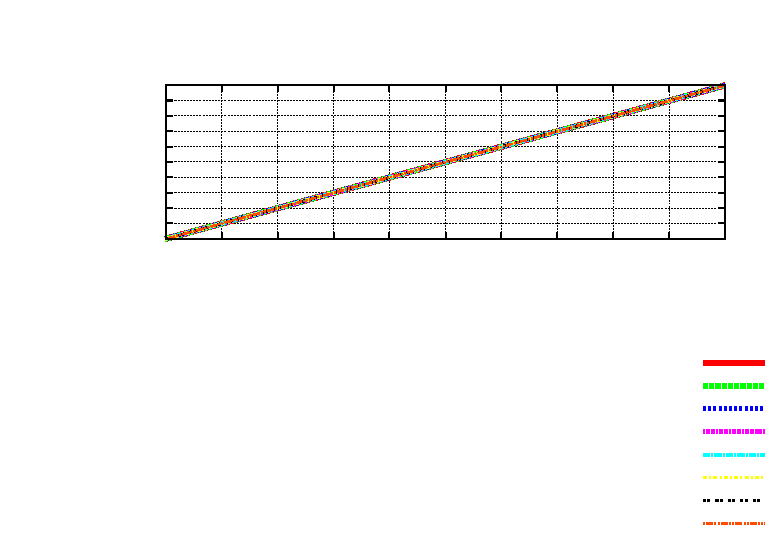
\includegraphics{ej3_frontera_complete_bipartite_sin_aspiracion_golosa}}%
    \gplfronttext
  \end{picture}%
\endgroup
}
    \caption{Frontera de grafos Bipartito Completo (sin aspiracion,golosa)}
\end{figure}

\subsubsection{Conclusiones}
\par En los resultados exhibidos no se han encontrado cosas particularmente
    destacables a\'un (esperamos encontrar estos resultados al comparar
    la b\'usqueda tab\'u con las dem\'as heur\'isticas y el algoritmo exacto).

\par En particular, nunca est\'a de m\'as advertir que las cotas de complejidad
    de peor caso se cumplieron en los resultados emp\'iricos obtenidos.

\par A\'un as\'i, los resultados expuestos no nos dicen demasiado sobre las
    diferentes variantes. Vale la pena notar que las variantes con
    funci\'on de aspiraci\'on requieren menos tiempo para terminar (esta
    es una comparaci\'on que se debe hacer mirando las escalas de los gr\'aficos
    correspondientes a las variantes con y sin funci\'on de aspiraci\'on).

\par Tambi\'en se nota, comparando de la misma manera que se expuso en el
    p\'arrafo anterior, como las variantes que tienen $MAX\_ITERACIONES$
    con la variante $n\cdot log(n)$ requieren muchas m\'as iteraciones
    para terminar con la b\'usqueda.

\par Por \'ultimo, ya comparando finamente, se puede observar que la variante
    con $n = MAX\_ITERACIONES$, $n/2 = SIN\_MEJORAR$ y $n/2 = TIEMPO\_TABU$
    requiere en varias de las familias expuestas una cantidad considerable
    menos de iteraciones para terminar, sin afectar negativametne (o no
    demasiad) su valor retornado respecto de las dem\'as.
